\documentclass[12pt]{report}
\usepackage[a4paper, total={6in, 8in}]{geometry}
\usepackage[utf8]{inputenc}
\usepackage[toc,page]{appendix}
\usepackage{cite}
\usepackage{graphicx}
\usepackage{caption}
\usepackage{subcaption}
\usepackage{indentfirst}
\usepackage{listings}
\usepackage{amsfonts,amssymb}
\usepackage{amsmath}
\usepackage{algorithm}
\usepackage[noend]{algpseudocode}

\usepackage{titlesec}
%\newcommand{\sectionbreak}{\clearpage}
\newcommand{\R}{\mathbb{R}}
\newcommand{\A}{\mathcal{A}}
\newcommand{\B}{\mathcal{B}}
\newcommand{\C}{\mathcal{C}}
\newcommand{\G}{\mathcal{G}}
\newcommand{\X}{\mathcal{X}}
\newcommand{\Y}{\mathcal{Y}}
\newcommand{\M}{\mathcal{M}}


\newcommand{\w}{{\mathbf{w}}}
\newcommand{\f}{{\mathbf{f}}}
\newcommand{\col}{{\col}}

\newcommand{\bmu}{{\boldsymbol{\mu}}}



%\theoremstyle{plain}% default
\newtheorem{thm}{Theorem}[section]
\newtheorem{lem}[thm]{Lemma}
\newtheorem{prop}[thm]{Proposition}
%\theoremstyle{definition}
\newtheorem{defn}{Definition}[section]
\newtheorem{conj}{Conjecture}[section]
\newtheorem{exmp}{Example}[section]


\newtheorem{theorem}{Theorem}[section]
\newtheorem{lemma}[theorem]{Lemma}
\newtheorem{proposition}[theorem]{Proposition}
\newtheorem{corollary}[theorem]{Corollary}

\newenvironment{proof}[1][Proof]{\begin{trivlist}
\item[\hskip \labelsep {\bfseries #1}]}{\end{trivlist}}
\newenvironment{definition}[1][Definition]{\begin{trivlist}
\item[\hskip \labelsep {\bfseries #1}]}{\end{trivlist}}
\newenvironment{example}[1][Example]{\begin{trivlist}
\item[\hskip \labelsep {\bfseries #1}]}{\end{trivlist}}
\newenvironment{remark}[1][Remark]{\begin{trivlist}
\item[\hskip \labelsep {\bfseries #1}]}{\end{trivlist}}

\newcommand{\qed}{\nobreak \ifvmode \relax \else
      \ifdim\lastskip<1.5em \hskip-\lastskip
      \hskip1.5em plus0em minus0.5em \fi \nobreak
      \vrule height0.75em width0.5em depth0.25em\fi}

\DeclareMathOperator*{\argmin}{arg\,min}
\DeclareMathOperator*{\vect}{vec}
\DeclareMathOperator*{\skw}{skew}
\DeclareMathOperator*{\tr}{tr}
\DeclareMathOperator*{\rk}{rank}
\DeclareMathOperator*{\im}{im}
\title{tensor_decomp_comparison}
\author{a.nigmetov }
\date{December 2013}

\begin{document}

\tableofcontents

% describe model
% 

%One of the approaches to tensor decomposition

%Bolkart and WuhrerIn the multilinear model from\cite{bolkart_wuhrer_2013} 


\chapter{Introduction}


The human face is, perhaps, the most important means of non-verbal 
communication, and there are numerous scenarios where
we need to analyze faces.
For example, the problem of expression recognition
attracted a lot of attention in the computer vision community,
and significant progress has been made.
% (see the survey by Sandbach et al. \cite{sandbach_2012}).
Computer graphics is interested in synthesizing realistic images 
of human faces or editing existing ones. In human-computer interaction,
if we wish to animate a virtual avatar so that it reflects the actual
emotions of a user, it is necessary to solve both these problems.
A similar example is provided by cinema industry,
where virtual characters get their mimic from real actors.
Another application can be editing photos to change the expression
of a person in this photo. 
For security applications it may be convenient to use
a face for identification purposes.
In ergonomics one studies the statistical distribution 
of shapes of faces to determine optimal design for face masks.


Some of these applications are naturally 3-dimensional (image synthesis
is rendering a 2D image of a 3D model),
some of them may become 3-dimensional in a short period of time (since 3D technologies become more and more accessible,
it might be that a 3D-scanner will be a part of standard laptop
in the future, as a web-camera is now). 


A popular approach to solve these problems 
is building a  statistical model. One acquires a large database of faces,
represents each face as a coordinate vector and studies
the distribution of these vectors. Of course, if we want
to apply statistical models to such a sample of vectors,
they all must have the same dimensionality and the points
on each scan must be in correspondence. This means
that as a preprocessing step it is necessary to \textit{register} 
all scans, that is, to establish dense correspondence between points.
It is also helpful, if the database is annotated, the information
can include gender, age, ethnicity, emotion, and position
of landmarks (certain keypoints, such as tip of the nose, corners of eyes,
etc) on each instance. It is clear that acquiring such a database involves a lot of work.
%is a challenging task,
Nevertheless, now there are several publicly available
databases of 3D face scans (e.g., BU-3DFE by Yin et al., \cite{BU_3DFE}, BU-4DFE by Yin et al.
\cite{BU_4DFE}, Bosphorus by Savran et al. \cite{Savran}).


In this thesis we shall work with one statistical
model which is called the multilinear model.
It is aimed at separating identity and expression variations
of 3D shape of a face, which is a desirable property in many applications 
(e.g., an automated surveillance system should recognize
a person independently of the person's mood).
The model  is based on a certain form
of compression of multidimensional arrays, a problem
that does not have a closed-form solution.
The first step of this projection procedure is to center
the data by subtracting the mean. 
The compression of the centered array is performed by applying orthogonal
projections along different dimensions of the array in order to get a 
new array whose dimensions are significantly smaller than the dimensions
of the original one. This new array is called a \textit{core}. The exact formulation
of the problem will be given in Chapter \ref{chap_mult_model}.


There are several approximate methods to estimate the optimal
projection operators.   The objective of this thesis is to investigate
the influence of the following four numerical algorithms
for solving this problem on the quality of the model: 
\begin{itemize}
\item Truncated Higher-Order Singular Value Decomposition (\cite{kolda_bader_2009});
\item Higher-Order Orthogonal Iteration (\cite{kolda_bader_2009});
\item Newton-Grassmann method (\cite{elden_savas_2009}) ;
\item Differential-Geometric Newton method (\cite{IDLAVH09}).
\end{itemize}
We should note that the multilinear model for faces requires one of the projection
operators to be fixed. This  difference in the problem formulation
leads to some modifications of the algorithms. For the first two algorithms
these modifications are easy to make and the corresponding versions of these 
algorithms have already been formulated in the literature.
However, the formulas for the last two algorithms are lengthy,
so it is necessary to derive them for the modified problem
following the derivations in the original papers.



The contributions of this thesis are:
\begin{itemize}
\item Modification of the Newton-Grassmann and Differential-Geometric Newton methods
for the problem formulation used in the multilinear model.
\item Actual implementation of all four algorithms.
\item Evaluation of the algorithms on facial data using the
standard numerical analysis criteria and some rough practical estimates of the running time.
\item Evaluation of the resulting models with two application-relevant
problems: fitting and expression recognition.
Fitting means that for an (unseen) face scan 
we are trying to generate the closest approximation
of this scan using the learnt model. This test measures
the ability of the model to \textit{generalize}.
In the expression recognition test we use the model
to classify the expression of the input face. Having a good
classification rate means that the model has successfully separated identity
and expression information.
\end{itemize}


The thesis is organized as follows. In Chapter \ref{rel_work}
we discuss related work. Then we formulate
the multilinear model in Chapter \ref{chap_mult_model}. 
In Chapter \ref{chap_algo} we discuss the four algorithms that we evaluate.
Chapter \ref{chap_eval} contains experimental evaluation results
and implementation details. The conclusion
is summarized in Chapter \ref{chap_conclusion}.


\chapter{Related Work}
\label{rel_work}


\section{Statistical Models and Their Applications}
The first statistical model for 3D faces
was introduced in Blanz and Vetter~\cite{BlanzVetter1999}. They worked with both texture and geometric data,
but most of the faces in their database were in neutral expression.
They used an optic flow technique to establish dense correspondence
between scans and then applied  principal
component analysis (PCA) to learn the low-dimensional subspace.
The learnt model was used to reconstruct $3D$ faces from $2D$ images
and to generate new faces. 



Let us briefly recall how PCA works using geometric 3D data as an example.
Blanz and Vetter represent each 3D face scan as a column vector $\mathbf{S}_i$
and arrange them in the matrix $S = [ \mathbf{S}_1 \, \dots \, \mathbf{S}_m ]$,
where $m$ is the number of faces. Let $\bar{\mathbf{S}}$ be the mean face (average of $\mathbf{S}_i$). 
We center the data by subtracting $\bar{\mathbf{S}}$ from each column of $S$,
let $A$ be the centered matrix.
If $U$ is a $k \times m$ matrix with orthonormal columns and $k < m$, 
we can compress the centered data using $U$,
\begin{equation}
\label{pca_compress1}
M = U A.
\end{equation}
Multiply both sides of the equation \eqref{pca_compress1} with $U^T$ from the right. 
Since $U$ has orthonormal columns, the matrix $U^T U $ is a diagonal matrix
with $k$ first diagonal entries equal to $1$ and all other entries being $0$. 
\begin{equation}
A \approx U^T M .
\end{equation}
We call the compressed matrix $M$ the \textit{core matrix}, and the projection $U$ is
called a \textit{factor matrix}.  If we want the restored version to be the closest
possible approximation of the original data, the PCA theory says 
that the projection matrix must consist of 
the eigenvectors of the covariance matrix that correspond to the largest eigenvalues (this eigenvectors 
This projection gives us the low-dimensional subspace that keeps as much variance as possible.
Now, if we have $k$ parameters $\w = (w_1, \dots, w_k) \in \R^k$, we can generate 
a new face using the formula
\begin{equation}
\label{face_gen_pca}
\mathbf{S} = \bar{\mathbf{S}} + M \times \w.
\end{equation}



Further application of PCA to statistical analysis of shapes
was done by Yang et al.~\cite{Yang_2011}. 
Their paper is devoted to the expression transfer problem.
In this problem we have two images ${Im}_1$ and ${Im}_2$ of
two persons $P_1$ and $P_2$. We want to edit the first image $\mathrm{I}_1$
so that the person $P_1$ in this image will have the same expression as the person $P_2$
in the image ${Im}_2$. Yang et al. solve this problem by
learning separate PCA models for each expression. 




Vasilescu and Terzopoulos \cite{vt_2002} 
proposed building a single statistical  model that decouples
variations for different identities
and expressions. They
used a generalization of PCA,
which is  applied  to multidimensional arrays.
They were inspired by the same approach in natural language processing,
where this idea was  used by Tenenbaum and Freeman \cite{Tenenbaum_2000} to decouple author 
and style of a text.
Vlasic et al.~\cite{vlasic}  generalized the bilinear model 
used by Vasilescu and Terzopoulos. They also applied their model
to the expression transfer problem. We shall use the multilinear model as it 
was formulated in~\cite{vlasic} in this thesis.  
Dale et al.~\cite{dale} applied the multilinear model to editing video 
sequences. Mpiperis et al.~\cite{mpip} introduced another variant
of a multilinear model and applied it to recognize both expression and identity
of a face. We shall use an approach similar to this method
 in our expression recognition experiments.



We postpone the formal definitions of all necessary notation to Chapter \ref{chap_mult_model}.
However, just to show that multilinear model is indeed a generalization 
of PCA, we give some basic formulas here.  Let $\X$ be a multidimensional
array in which we organize our data (e.g., dimension 1 corresponds to the coordinates
of vertices, dimension 2 corresponds to the identity and dimension 3 corresponds to the expression).
Such arrays will be called 
\textit{tensors}.
As in PCA, we need to center the data by subtracting the mean face $\bmu$ from each scan, let $\A$
denote the centered array.
The multilinear model consists of the
\textit{core tensor} $\G$ and projection matrices $F_2$ and $F_3$ with orthonormal columns such that

\begin{equation}
\label{tucker_prelim}
\Y  \approx \G \times_2 F_2^T \times_3 F_3^T .
\end{equation}

Now, if we have two vectors $\w_2$ and $\w_3$, we can generate a new face by
\begin{equation}
\label{face_gen_mlm}
\f = \bmu + \G \times_2 \w_2^T \times_3 \w_3^T.
\end{equation}

The exact meaning of the notation used in these formulas is explained in the next chapter. However,
the reader can immediately spot certain similarity between formulas \eqref{face_gen_pca}
and \eqref{face_gen_mlm}.

A further generalization of the multilinear model was proposed by Brunton et al. \cite{brunton_mwave}.
Instead of one model that captures the whole face they learn several multilinear
models for different scales. The authors use wavelets to perform localization.
As a side remark we should note that there is a theoretical justification 
by Xu and Chowdhury~\cite{xu2008} for using localized linear and multilinear models for 2D images.
However, no such justification is known for 3D data.


There are a lot of papers which apply linear or multilinear statistical models 
in various scenarios. For example, the morphable model by Blanz and Vetter
was used in \cite{Blanz2007} for face recognition (with restriction to neutral expression) and for registration
of 3D scans. Registration with morphable model was also performed by Patel and Smith \cite{PatelSmith2009}.
The multilinear model formulated by Vlasic et al. \cite{vlasic} was used by Bolkart and Wuhrer \cite{BolkartWuhrer2014} to analyze motion data (the motion sequences were automatically registered, there also are applications
to the synthesis of new motion sequences and dynamic expression recognition).
We have already mentioned expression transfer problem. 

\section{Tensors and Tensor Decompositions}

Multilinear model is based on the compression of multidimensional arrays
of the form \eqref{tucker_prelim}. Multidimensional arrays
are called tensors and this form of compression is called Tucker decomposition. It was introduced by Ledyard L. Tucker  \cite{tucker_63} in 1963 and was originally applied to psychometic problems.
The first method of computing this decomposition was proposed by Tucker himself and
is now known as truncated higher-order singular value decomposition. We shall refer to it
as HOSVD, it is described in Section \ref{sec_hosvd}.


The next algorithm was based on alternating least squares
approach and was called TUCKALS (Tucker Alternating least squares). It was developed
by Kroonenberg and De Leeuw \cite{kroonenberg}. Its further improvements
lead to a simple and fast iterative algorithm by De Lathauwer et al. \cite{de2000best}
known as higher-order orthogonal iteration (HOOI). We describe this algorithm in Section \ref{sec_hooi}.


These algorithms were developed using classical methods based 
on calculus and matrix algebra.  However, in the last decades
numerical linear algebra started using some more recent
tools of pure mathematics, especially differential geometry. There
are papers on optimization on Riemannian manifolds
in general (e.g., Adler et al. \cite{adler_spine}) or
papers studying optimization on specific classical manifolds. From the linear algebraic perspective, the most 
important examples of manifolds  are Stiefel 
and Grassmann manifolds (we shall explain later, why Grassmann manifold
is a natural domain to consider  Tucker decomposition
problem). The first paper devoted to optimization
on Grassmann manifolds was Edelman et al. \cite{edelman_1998}. It provided
a general geometric framework that allowed generalization
of well-known optimization algorithms in $\R^N$ to Grassmann manifolds (they also
considered Stiefel manifolds, but this is less relevant to us).
  This framework was used by Elden and Savas \cite{elden_savas_2009}
to develop a generalization of Newton method for Tucker decomposition problem which they 
called Newton-Grassmann method. This method operates on Grassmann manifold
and updates of factor matrices are performed by moving along the geodesic curves on this manifold.


Another generalization of the Newton method was proposed in Ishteva et al. \cite{IDLAVH09},
who work on a non-classical manifold that we shall introduce in Section \ref{sec_dg_newton}.
The manifold they work on is a quotient of the manifold of all $n \times p$ matrices
with maximal rank. The update of the factor matrices is performed
by simple addition. The algorithm is described in Section \ref{sec_dg_newton}.



Finally, we mention several papers that deal with some other forms
of decomposition or assume that the tensor has some special structure: \cite{elden_krylov},
\cite{badeau},  \cite{oseledets}, \cite{hao_horesh}.
There are also papers that introduce new algebraic operations on tensors and 
use this operations to define new types of decomposition, which are applied
in facial recognition and image deblurring: Kilmer et al. \cite{kilmer_3rd}, Hao et al. \cite{hao_kilmer}.


\chapter{Tensors and Multilinear Model}
\section{Tensor Notation}
% tensor notations
Notation we use here is mostly taken from ~\cite{elden_savas_2007} and ~\cite{kolda_bader_2009}.


By tensors we mean multidimensional arrays, that is, sets of real numbers 
$ \X = \{\X_{i_1 i_2 \dots i_n} \} $ indexed by sets $1 \leq i_j \leq I_j$.
The number of dimensions $n$ is called the order of the tensor, such tensors 
are also called $n$-way tensors.
Sometimes it will be more convenient to use Matlab-like notation. For example, if we have a matrix $M \in R^{I_1 \times I_2}$ and $1 \leq a < b \leq I_1$, the submatrix
of $M$ obtained by 'cutting out' rows from $a$ to $b$ is denoted by $M(a:b, :)$. The meaning of 
 $M(:, c:d)$ and $M(a:b, c:d)$ is also clear (of course, $1 \leq c < d \leq I_2$).
 


The set of all tensors with fixed dimensions $I_1$, $I_2$, $I_3$ is denoted by 
${\R}^{I_1 \times I_2 \times I_3}$. It has a natural structure of a vector space
with the canonical inner product defined by
\begin{equation}
    \langle \A, \B \rangle = \sum_{i_1 = 1}^{I_1}  \sum_{i_2 = 1}^{I_2} \sum_{i_3 = 1}^{I_3}  \A_{i_1, i_2, i_3} \B_{i_1, i_2, i_3}.
\end{equation}
The norm of the tensor defined by this tensor product is called a Frobenius norm:
\begin{equation}
    \| \A \| = \sqrt{ \langle \A, \A \rangle }.
\end{equation}


Matrices can be considered as ordered sets of vectors in two natural ways: they have
rows and columns. In the same way, tensors of order $3$ have $I_2 I_3 $ mode-$1$ fibers which
are elements of $\R^{I_1}$, $I_1 I_3$ mode-$2$ fibers (vectors from $\R^{I_2}$), and $I_1 I_2$ mode-$3$
fibers (vectors from $\R^{I_3}$).



Let $A$ be a $J \times I_1$ matrix $A$. If we multiply a mode-$1$ fiber of $X \in \R^{I_1 \times I_2 \times I_3}$ by $A$,
we get a vector from $\R^J$. Doing this with every fiber, we get a new tensor from $\R^{J \times I_2 \times I_3}$. It is denoted by 
$\X \times _{1} A$ and called a mode-$1$ product of $\X$ and $A$. In the same way we define mode-$k$ product. Namely,
if $A \in \R^{J \times I_k}$, then $\X \times_k A$ is a tensor defined by
\begin{equation}
    (\X \times_k A)(i_1, \dots, i_{k-1}, j, i_{k+1}, \dots, i_n) = \sum_{i_k = 1}^{I_k} \X(i_1, \dots, i_n) A(j, i_k).
\end{equation}
This operation has the following properties:
\begin{enumerate}
\item The products in different modes commute:
\begin{equation}
n \not= m \Rightarrow (\A \times _n B) \times_m C = (\A \times _m C) \times_n B.
\end{equation}
\item The product in one mode is associative:
\begin{equation}
(\A \times_n B) \times_n C = \A \times_n (BC).
\end{equation}
\item Orthogonal factors preserver Frobenius norm:

\begin{equation}
\label{orthogonal_norm_inv}
S \in O(I_k)  \Rightarrow \| \A \times_k S \| = \| \A \|.
\end{equation}
\end{enumerate}

There is a natural way of transforming tensor $\X \in R^{I_1 \times I_2 \times \cdots \times I_N}$ into a matrix: choose one mode $n$
and arrange all mode-$n$ fibers into a matrix in a natural order. More formally,
the unfolding in mode $n$ is an $I_n \times \prod_{k \neq n} I_k$ matrix such that
the element $X_{i_1 \dots i_N}$ is mapped to the row $i_n$ and column $j = 1 + \sum_{ k \neq n} (i_k - 1) J_k$,
with $J_k = \prod_{ m \in \{ 1, \dots, k-1 \} \\ {n} } I_m$.
 Unfolding  is a special case of \textit{matricization}. In general, in order to get a matrix
from $\X$ we fix the modes $\mathbf{r} =  (r_1, \dots, r_L)$ that will be mapped to rows.
Here $1 \leq r_i \leq n$ are distinct numbers. The other $M = n - L$  modes will be mapped
to columns $\mathbf{c} = (c_1, \dots, c_M)$.
The element $\X(j_1, \dots, j_n)$ is mapped to $X^{(\mathbf{r};\mathbf{c})}(j, k)$, where
\begin{eqnarray}
    j = 1 + \sum_{l = 1}^{L} ( i_{r_{L-l+1}} - 1) \prod_{l' = 1}^{l - 1} d_{r_{L - l' + 1}}, \\
    k = 1 + \sum_{m = 1}^{M} ( i_{r_{M-m+1}} - 1) \prod_{m' = 1}^{m - 1} d_{r_{M - m' + 1}}.
\end{eqnarray}
We illustrate the general formula with two specific examples
for a $4$-way tensor (we shall need these examples in Newton-Grassmann method).

If $\X \in \R^{I_1 \times I_2 \times I_3 \times I_4}$, then $\X^{(1,3;2,4)}$ is a 
matrix with $I_1 I_3$ rows and $I_2 I_4$ columns obtained by the following rule:
an element $\X(i_1, i_2, i_3, i_4)$ goes to the row $i$, column $j$ of $\X^{(1,3;2,4)}$,
where 
\begin{eqnarray}
i = 1 + (i_3 - 1) + (i_1 -1) I_3 \\
j = 1 + (i_4 - 1) + (i_2 -1) I_4.
\end{eqnarray}
The order of indices in $\mathbf{r}$, $\mathbf{c}$ is significant: the second matricization
we shall need is $\X^{(1,3;4,2)}$. The formulas for this variant are
\begin{eqnarray}
i = 1 + (i_3 - 1) + (i_1 -1) I_3 \\
j = 1 + (i_2 - 1) + (i_4 -1) I_2 
\end{eqnarray}



Let $\A \in \mathbb{R}^{I_1 \times \cdots \times I_k} $ and $\B  \in \mathbb{R}^{J_1 \times \cdots \times J_m}$ be tensors.
Their \textit{tensor product} is the tensor $ \A \otimes B  \in {\R}^{I_1 \times \cdots \times I_k \times J_1 \times \cdots \times J_m } $
defined by
\begin{equation}
    (\A \otimes B)(i_1, \dots, i_k, j_1, \dots, j_m) = \A(i_1, \dots, i_k) B(j_1, \dots, j_m).
\end{equation}
If $I_{\kappa} = J_{\mu}$, we define the \textit{contracted product} $\C = \langle \A, \B \rangle_{\kappa; \mu} $ of $\A$ and $\B$ in dimensions $\kappa$, $\mu$ as a tensor
obtained from $\A \otimes \B$ by 'summing out' in modes $I_{\kappa}$ and $J_{\mu}$, that is,
%\in {\R}^{I_1 \times \cdots I_{\kappa - 1} \times I_{\kappa +1} \times \cdots \times I_k \times J_1 \times  \cdots \times J_m } 
\begin{eqnarray}
    \C(i_1, \dots, i_{\kappa-1}, i_{\kappa + 1} , \dots, i_{k}, j_1, \dots, j_{\mu - 1}, j_{\mu+1}, \dots, j_{m}) = \notag\\
    \sum_{t = 1}^{I_{\kappa}} (\A \otimes \B)(i_1, \dots, i_{\kappa-1}, t, i_{\kappa+1}, \dots,  i_k, j_1, \dots, j_{\mu-1}, t, j_{\mu+1}, \dots, j_m).
\end{eqnarray}
If $I_{\kappa_1} = J_{\mu_1}$ and $I_{\kappa_2} = J_{\mu_2}$, then we can contract
by summing out in two pairs of modes in the same way. This contracted product is 
denoted $\langle \A, \B \rangle_{\kappa_1, \kappa_2; \mu_1, \mu_2}$.



If $\A$ and $\B$ are of the same order ($k = m$), then the notation is more compact.
If $\kappa = \mu$, then the contracted product
$\langle \A, \B \rangle_{\kappa; \kappa}$
is denoted by $\langle \A, \B \rangle_{\kappa}$. Analogous notation $\langle \A, \B \rangle_{(\kappa_1, \kappa_2)}$ is equivalent to $\langle \A, \B \rangle_{(\kappa_1, \kappa_2;\kappa_1, \kappa_2)}$.
The minus in $\langle \A, \B \rangle _{ -(\kappa_1, \dots, -\kappa_p)}$ means 
that contraction is performed in all modes but $\kappa_1, \dots, \kappa_p$. The following examples 
illustrate these definitions.


If $\A, \B \in \R^{I_1 \times I_2 \times I_3 \times I_4}$, then
\begin{eqnarray*}
\begin{split}
\langle \A, \B \rangle_{(2,3)} & \in \R^{I_1 \times I_4 \times I_1 \times I_4} \\
\left( \langle \A, \B \rangle_{(2,3)}\right)(i_1, i_4, j_1, j_4) &= \sum_{i_2 = 1}^{I_2} \sum_{i_3 = 1}^{I_3} \A(i_1, i_2, i_3, i_4) \B(j_1, i_2, i_3, j_4) \\
\langle \A, \B \rangle_{-3)} &= \langle \A, \B \rangle_{(1,2,4))} \in \R^{I_3 \times I_3} \\
\left( \langle \A, \B \rangle_{-3)}\right)(i_3, j_3) &= \sum_{i_1 =1 }^{I_1} \sum_{i_2 = 1}^{I_2} \sum_{i_4 = 1}^{I_4} \A(i_1, i_2, i_3, i_4) \B(i_1, i_2, j_3, i_4) 
\end{split}
\end{eqnarray*}


\section{Tucker Decomposition}


Suppose that we want to compress a tensor: instead of $\A \in \R^{d_1 \times d_2 \times d_3}$
we want to store only $\G \in \R^{r_1 \times r_2 \times r_3}$, where $r_k \leq d_k$.
The compression is performed by applying projections to a lower-dimensional
space in each mode, so that
\begin{equation}
    \G = \X \times_1 F_1 \times_2 F_2 \times_3 F_3, \quad F_i \in \R^{r_i \times d_i}.
\end{equation}
Though it  is not necessary to impose any constraints on the  projection matrices $F_i$,
it is usually assumed that they have orthonormal columns. In this case it is
easy to restore the approximate version of $\X$ from $G$:
\begin{equation}
    X \approx G \times _{1} F_1^T \times _{2} F_2^T \times _{3} F_3^T.
\end{equation}
This approximation is called Tucker decomposition. 
As a side remark we notice that there is a specific case of Tucker decomposition
called CP. The minimal number of components (they are \textit{rank-1 tensors}) needed
in CP decomposition to exactly represent $\X$ is called \textit{the rank of $\X$},
finding this rank is an NP-hard problem (\cite{}).



We shall use a variant of Tucker decomposition (known as Tucker2)
in which we do not compress in mode $1$, so $F_1$ is fixed to be
identity matrix.  
The quality of approximation can be measured by the Frobenius norm of the residual $\| \X - \G \times _{1} F^T_1 \times _{2} F^T _2 \times _{3} F^T_3$,
so the best Tucker2 decomposition is a solution of
the following optimization problem:
\begin{equation}
    \label{tucker_min}
\| \X - \G \times_2 F_2^T \times_3 F_3^T \| \to \min
\end{equation}
where $F_2$ and $F_3$ are matrices with orthonormal columns.
The following equality holds:
\begin{equation}
\label{tucker_min}
\begin{split}
    \| \X - \G \times_2 {F_2^T} \times_3 {F_3^T} \|^2  &= \| \X \|^2 - \| \G \|^2 \\
                                                       & = \| \X \|^2 - \| \X \times_2 {F_2} \times_3 {F_3} \|^2.
\end{split}
\end{equation}
In particular, this equality proves that the Frobenius norm
of the compressed version of $\X$ ('energy') cannot be greater than the norm
of the original tensor $\X$. It also shows that the best decomposition
is a solution of the maximization problem
\begin{equation}
\label{tucker_max}
\Phi(F_2, F_3) = \frac{1}{2} \| \X \times_2 F_2 \times_3 F_3 \|^2 \to \max.
\end{equation}
Since the set of matrices with orthonormal columns is compact,
this problem is guaranteed to have a solution.
The property \eqref{orthogonal_norm_inv} implies that
for all orthogonal matrices $S_2 \in O(d_2)$, $S_3 \in O(d_3)$
\begin{equation}
    \Phi(F_2 S_2, F_3 S_3) = \Phi(F_2, F_3),
\end{equation}
so the best Tucker2 decomposition is not unique. 
The geometric interpretation of this fact
is that we are actually looking for subspaces
the projection to which preserves as much energy
as possible, and the exact projection operators
given by $F_i$ matrices do not matter, it is 
just another choice of the basis in the same subspace.


\section{Multilinear Model}


This thesis uses the multilinear model as it is formulated in \cite{bolkart_wuhrer_2013}.
Suppose that we have a registered set of face scans of different people expressing different
emotions.

The registration process must ensure that all scans have the same number of points
and these points must be in dense correspondence to each other, otherwise
it would not make sense to apply statistical methods
to the data. It is also necessary to have full set of expressions for each 
person (we do not consider the problem of restoring missing data).

We can organize these data in a $3$-way tensor. Mode $1$ corresponds
to coordinates, mode $2$ is identity, and mode $3$ is expression.
To this end, we flatten each scan: if $(p_1, \dots, p_n)$ is a set of points in $R^3$, then we write
the coordinates of all points into one vector $(p_{1, x}, p_{1, y}, p_{1, z}, \dots, p_{n, x}, p_{n, y}, p_{n, z}$
and take this vector as mode-$1$ fiber of the tensor $\Y$. The fibers $\Y(:, i, j)$
and $\Y(:, i', j)$ represent different persons with the same expression, the fibers
$\Y(:, i, j)$ and $\Y(:, i, j')$ are scans of the same person performing different expressions. 
The tensor $\Y$ has dimensions $d_1$, $d_2$, $d_3$, where $d_1 / 3$ is the number
of points in each scan, $d_2$ is the number of people, and $d_3$ is a number
of expressions.



The first step is to calculate the \textit{mean face} $\bmu$,
\begin{equation}
    \bmu := \frac{1}{d_2 d_3} \sum_{i_2, i_3} \Y(:, i_2, i_3).
\end{equation}
Then we subtract $\bmu$ from all mode-$1$ fibers and get a centered tensor $\X$, 
which is compressed using Tucker2 decomposition for some $r_2 < d_2$, $r_3 < d_3$,
\begin{equation}
    \X \approx \G \times_2 F_2 \times_3 F_3.
\end{equation}



This is a generative model. If we choose $\mathbf{w}_2 \in \R^{r_2}$,
$\w_3 \in \R^{r_3}$, we can generate a new face
\begin{equation}
    \label{mlm_generate}
    \f(\w_2, \w_3) = \bmu +  \G \times_2 \w_2 \times_3 \w_3
\end{equation}
The idea is that by changing $\w_2$ we should get a face of another person
with the same expression, by changing $\w_3$ we keep the identity
and change only the expression. Therefore $\w_2$ is called \textit{identity weights}
and $\w_3$ is \textit{expression weights}.

If we are given a face scan $\tilde{\f}$, we can look for $\w_2$, $\w_3$ such that
$\f(\w_2, \w_3)$ is the best approximation  of $\tilde{\f}$. 



As a final remark we note that this model is a generalization of Principal Component 
Analysis. In PCA we are looking for a subspace projection to which
preserves as much variation as possible, that is, we approximate
the (centered) data with a linear subspace.
In multilinear model we are looking for two subspaces and perform projection
in different modes. If we fix expression, the multilinear model
also gives us a linear (or, more precisely, an affine) subspace that approximates 
the set of faces with  this expression. Indeed,
the equation \eqref{mlm_generate} for fixed $\w_3$ is a parametric
equation of an affine subspace. However, when we change
expression, this subspace changes in a linear fashion. Of course,
expression and identity play symmetric roles.


\chapter{Algorithms for Computing Tucker2 Decomposition}
\label{chap_algo}

\section{Mathematical Preliminaries}

In this section we recall some mathematical notions
we shall need to discuss the last two algorithms, 
Newton-Grassmann and Differential-Geometric Newton methods.

\subsection{Newton's method}

Let us recall some basic facts about ordinary Newton method. The minimization problem for 
a smooth function is usually reduced to finding zero of the gradient, 
so we shall discuss solving system of equations
$f(x) = 0$, $f \colon \R^n \to \R^n$.

 Geometrically the idea of the method in one-dimensional case is 
to move along the tangent lines to the graph of $f$. Analytically this is expressed by the following iterative formula:
\begin{equation}
 x_{n+1} = x_n - \frac{f(x_n) }{ f'(x_{n})}. 
\end{equation}


\begin{figure}
        \centering
                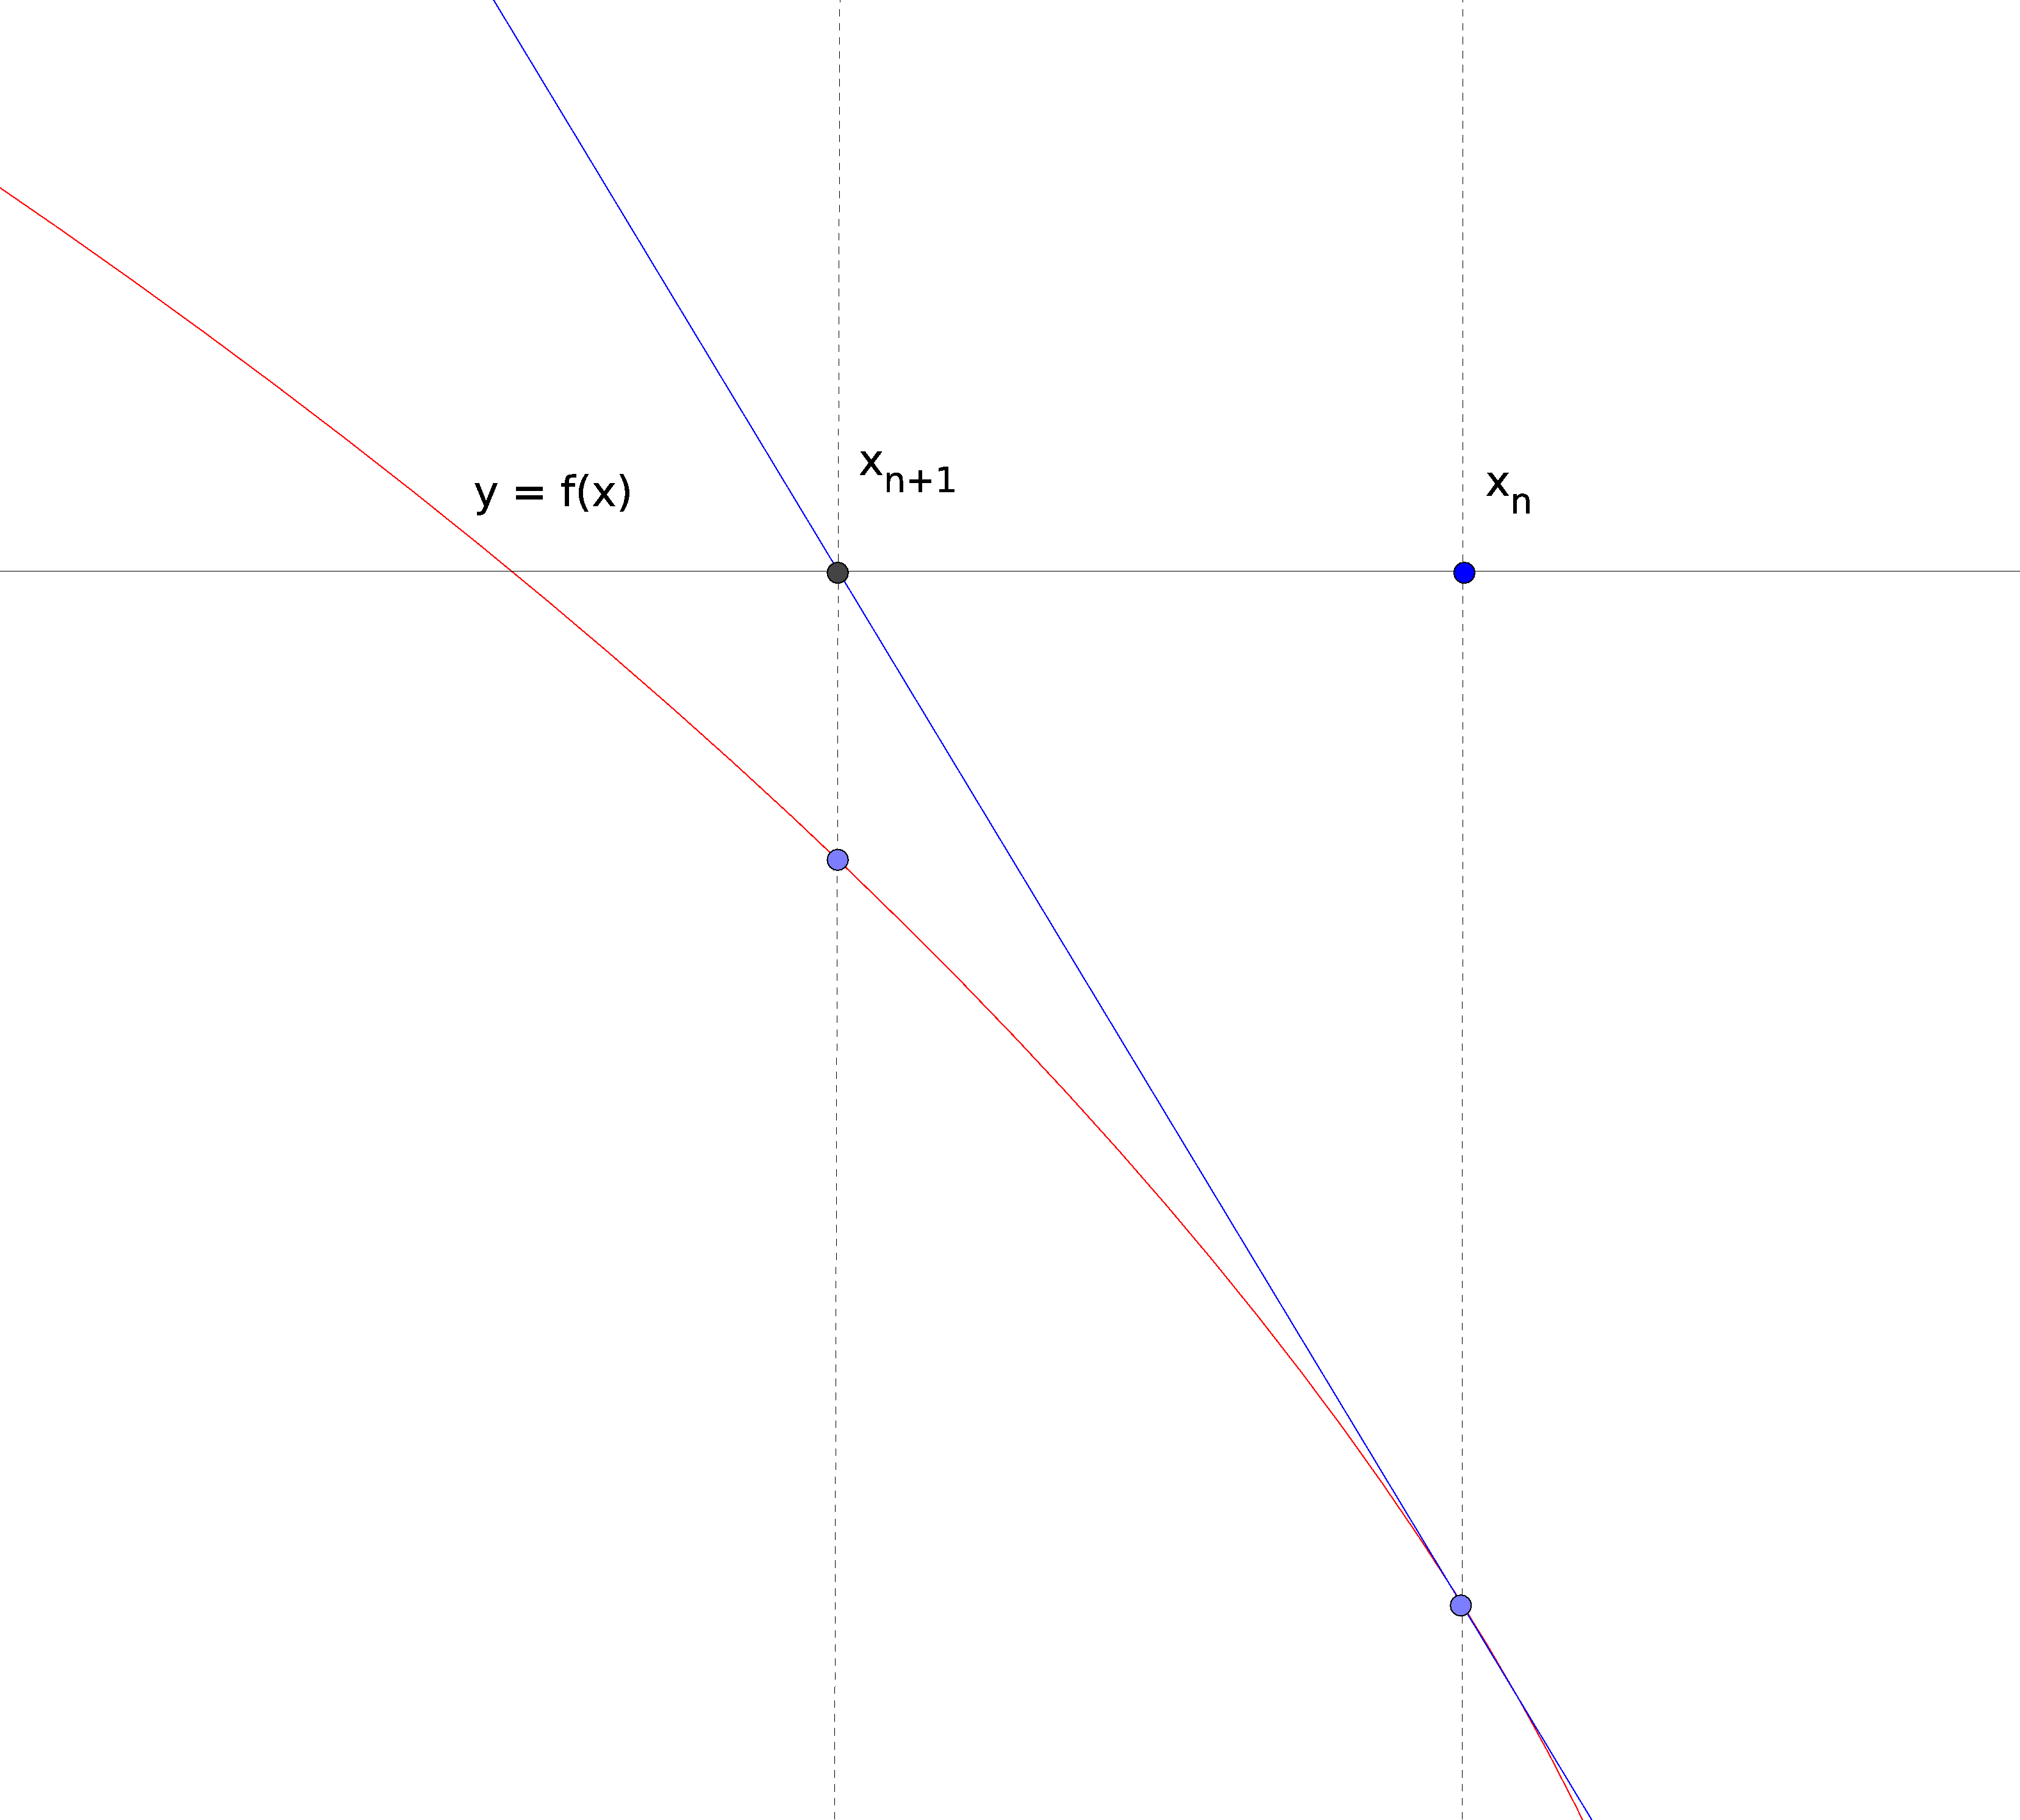
\includegraphics[width=8cm]{images/newton-image1.png}
        \caption{Newton's method illustration}
        \label{fig:hooi_hosvd_comparison}
\end{figure}
The method is known to be very fast-convergent (providing that the initial value $x_0$ is close enough to a root).
In multidimensional case the formula is
\begin{equation}
 x_{n+1} = x_n - ((Df)(x_n))^{-1} ( f(x_n) ).
\end{equation}
Here $(Df)(x_n)$ denotes the Jacobi matrix of the mapping $f$. In practice, instead of finding
the inverse of this matrix and then applying it to the vector $f(x_n)$, it is 
easier to solve the linear system $(Df)(x_n) y = f(x_n) $, but still this step is computationally expensive,
especially if the number of variables is high.


If we use this method to minimize $F$ by finding the zero of $\nabla F$, then
we can also interpret this method in terms of $F$. If we approximate $F$
with its Taylor expansion of degree $2$, then in a neighbourhood 
of a non-degenerate extremum point the level sets will be ellipses.
The gradient is known to be orthogonal to level set, so, if we use gradient descent,
we may come to the optimum quite slowly, if the ellipses are very elongated.
The Newton's method involves inverting of $D (\nabla F)$, that is, inverting 
the Hessian of $F$, which is exactly the quadratic part of the Taylor expansion.
By inverting it we essentially transform our problem to a coordinate system in which
the level sets are circular and this allows us to move to the optimum much faster (see Figure \ref{fig:newt_grad_comp}).

\begin{figure}
        \centering
                
\includegraphics[width=4cm]{images/newton_vs_grad_desc.jpg}
        \caption{Newton's method illustration}
        \label{fig:newt_grad_comp}
\end{figure}


However, Newton's method is known to behave poorly, if the root is not isolated.
This is exactly the situation we have in Tucker2 decomposition, where the objective function
does not change, if factor matrices are multiplied by any orthogonal matrices. The geometric
interpretation of this operation is that we choose another orthonormal basis in the same subspace.
There are orthogonal matrices approximately close to the identity matrix, so the zeros
of gradient w.r.t. entries of $F_2$, $F_3$ are not isolated. In order to apply Newton's method
we need to work in more geometric terms, and we start by brief informal description of the notions
that are necessary, namely: smooth manifold, tangent space, differential of a mapping between two smooth manifolds,
Riemannian metric, geodesic.
We are not going to give 
rigorous mathematical definitions, otherwise it would be necessary
to reproduce a significant part of several mathematical textbooks.
Instead we give a very informal description, which should be sufficient
to understand the intuition behind the two remaining methods.


\subsection{Some notions from differential geometry}
A smooth manifold of dimension $n$ is a space which locally 
looks like $\R^n$. 
This means that in a neighbourhood of each point we have a local coordinate system $(x_1(\cdot), \dots,  x_n(\cdot))$.
Point $p$ of a manifold $M$ in this system is described by $(x_1(p), \dots, x_n(p)) \in \R^n$. Usually these coordinate systems 
cover only a part of the manifold, but each point belongs to the domain
of at least one of them.
If the domains of two coordinate systems $(x_1(\cdot), \dots, x_n(\cdot))$
and $(y_1(\cdot), \dots, y_n(\cdot))$ intersect, then we have transition functions
\begin{equation}
(x_1, \dots, x_m) \mapsto (y_1, \dots, y_n) \mbox{ if } \exists p : x_i(p) = x_i \mbox{ and } y_i(p) = y_i \mbox{ for all } i.
\end{equation}
These functions must be differentiable (this is a part of the definition of smooth manifold).
This approach to manifolds does not require them to be a subset of 
any ambient Euclidean space $\mathbb{R}^N$. There is Whitney's embedding theorem 
that states that any manifold can be embedded into $\mathbb{R}^N$
for some $N$. However, sometimes there is no good or natural way to choose this embedding.
Examples.
\begin{enumerate}
    \item $\R^n$ is a manifold (the identity mapping is a coordinate system that
        covers the whole space). Since every finite-dimensional vector space is 
        isomorphic to $\R^n$, vector spaces are also manifolds. In particular,
        the space of $m \times n$ matrices is a manifold isomorphic to $\R^n$.
    \item If $M$ is a manifold, then every open subset of $M$ is also a manifold.
        In particular, the set of $m \times n$ matrices with some fixed rank $k$
        is a manifold. We shall need the set $\R^{n \times n}_{*}$ of non-singular $n \times n$ matrices,
        which is a manifold by this remark.
    \item If $M$ is a smooth manifold and there is an equivalence relation $\sim$ on $M$,
        then, under some conditions, the set of equivalence classes $M / \sim$ is 
        also a manifold (\textit{quotient manifold theorem}, see \cite{lee_manifolds}).
    \item If $M$ and $N$ are smooth manifolds, then $M \times N$ is a smooth
        manifold.
\end{enumerate}


Let $p$ be an arbitrary point of a smooth manifold $M$. The tangent space at $p$
is a vector space of the same dimension as $M$ and it is denoted by $T_pM$.
Suppose that for each point $p \in M$ we choose one vector $X_p \in T_pM$. 
This gives us a mapping $X: M \to \cup_{p \in M} T_pM$ called a
\textit{vector field on $M$}.


The notion of a tangent space is intuitively clear if we think about something like a sphere.
However, if $M$ is an open subset of $\R^n$, the tangent space at each point
is also $\R^n$.
\begin{equation}
    \forall p \in \R^n \quad T_p\R^n = \R^n.
\end{equation}
We shall often use this in the discussion of Newton methods, because
it allows us to treat matrix-valued functions of matrix argument $\R^{m \times n} \to \R^{m \times n}$
as vector fields on the manifold of matrices ($\R^{m \times n} \cong \R^{mn}$ as vector spaces).


Generally speaking, the only structure that $T_pM$ has is that of a vector space, there is no
inner product and there is no correspondence between $T_pM$ and $T_qM$ for different
points $p, q \in M$. However, this structure is sufficient to define a differential
of a mapping between two smooth manifolds. Let $f : M \to N$ be a smooth
function between smooth manifolds $M$ and $N$ (this means that, if we write
$f$ in local coordinates on some part of $M$ and the corresponding part of $N$,
we get a smooth function of real arguments). The differential of $f$
at point $p \in M$ is a linear operator $(Df)_p : T_pM \to T_{f(p)}N$ which in
local coordinates is given by the Jacobi matrix. In particular,
if $f : M \to \R$ is a smooth real-valued function on $M$, its differential at point $p$,
called \textit{gradient} is a linear functional on $T_pM$,
so the gradient of a function is not a vector (element of a tangent space),
but a covector (element of an adjoint space $(T_pM)^*$).



If each $T_pM$ is equipped with an inner product
that changes smoothly as we move along $M$, then $M$ is said to be a Riemannian manifold.
A smooth curve on $M$ is a smooth mapping $\gamma : [a, b] \rightarrow M$.
Its differential at point $p \in (a, b)$ is a linear mapping $(D\gamma)(p) : T_p(a,b) \to T_pM$.
By the previous remark, $T_p(a, b) = T_p \R = \R$, and we can calculate $(D\gamma)_p(1) \in T_pM$.
This element of $T_pM$ is called \textit{velocity vector}, and we can calculate
its Euclidean norm using the inner product in $T_pM$. This defines a real-valued function
on $(a, b)$. By definition, the length of the curve $\gamma$ is the integral
of this function over $(a,b)$, so the Riemannian structure allows us to measure curves on $M$.


Moreover, if $T_pM$ has an inner product, then there is a natural isomorphism
between $T_pM$ and its adjoint space $(T_pM)^*$. This means that the 
gradient of a function on a Riemannian manifold can be viewed as a vector (element
of $T_pM$).


If two different points $p, q$ on a Riemannian manifold are close enough to each other,
there is a unique shortest path connecting $p$ and $q$. 
The condition of being locally shortest path is certain differential equation
and it's solutions are called geodesics. If we consider $S^2$ in $\mathbb{R}^3$, 
then geodesics are arcs of large circles. This example illustrates that in general it is not true,
that two points are connected by the unique geodesics (consider North and South poles)
or that geodesic path is always the shortest: if $p$ and $q$ are close to each other,
there is a unique large circle passing through $p$ and $q$, but it gives rise to two
geodesics: the shortest path is the shorter arc of the circle, but the longer arc 
is a geodesic, too.


In the differential-geometric Newton method
we shall need the notion of fiber bundle.
We start with two toy examples.
A cylinder $ \{ (x, y, z) \mid x^2 + y^2 = 1, 0 \leq z \leq 1 \}$
can be split into disjoint copies of $[0,1]$ (generating lines)
parameterized by the base $\mathbb{S}^1$,
so there is one instance of $[0,1]$ attached to each point of the circle.
A M\"obius band can also be split into disjoint segments
$[0,1]$ parameterized by $\mathbb{S}^1$. Locally both the cylinder
and M\"obius band are isomorphic to a cartesian product
of the arc of a circle and $[0,1]$. The cylinder is, of course,
isomorphic to the cartesian product not just locally, but globally,
but it is not the case for the M\"obius band, where the trivial
 pieces are glued together in a non-trivial way. Both these spaces
are called total spaces of fiber bundles with the base $\mathbb{S}^1$ and fiber $[0,1]$.
Another example of a fiber bundle is a torus $\mathbb{S}^1 \times \mathbb{S}^1$,
where both the base and the fiber are circles. 

In general, a fiber bundle is a triple $( \pi, E, B)$, where
$ \pi \colon E \to B$ is a surjective mapping such that:
\begin{enumerate}
    \item The inverse image $\pi^{-1}(p)$ of each point $p \in B$ is 
    isomorphic to some fixed manifold $F$.
    \item Every point $p \in B$ has a neighbourhood $V_p$
    such that $\pi^{-1}(V_p)$ is isomorphic to $V_p \times F$.
\end{enumerate}
    The space $E$ is a \textit{total space} of the bundle, $B$ is a textit{base}, and $F$ is a \textit{fiber}.

Since the tangent space is a local notion, for each point $p \in E$
the tangent space at $p$ is isomorphic to a direct product
of the tangent space to the base $T_h$ and the tangent space to the fiber $T_v$,
\begin{equation}
    T_p E = T_h \oplus T_v
\end{equation}
If one wants to visualize a fiber bundle,
one usually thinks of the base positioned horizontally and the fibers
attached to the base in the orthogonal (that is, vertical) direction,
therefore the space $T_h$ is called a horizontal space and the space $T_v$
is called a vertical space.

\begin{figure}
        \centering
                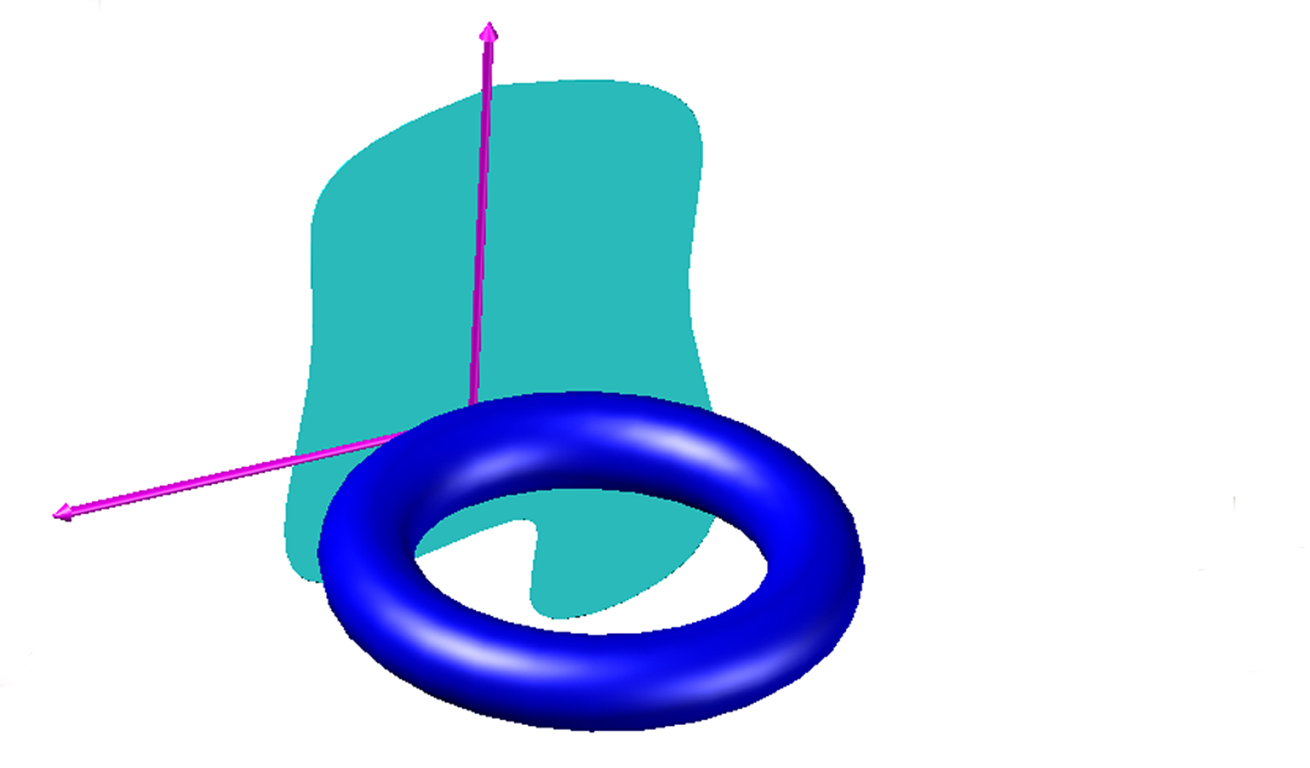
\includegraphics[width=8cm]{images/torus_tangent.jpg}
        \caption{Tangent plane to a fiber bundle}
        \label{fig:torus_tangent}
\end{figure}


The last notion we shall describe here is \textit{affine connection on a manifold}.

We say that $\nabla$ is an affine connection on a manifold $M$,
if for each vector field $X$ on $M$ we have an operator $\nabla_X$ that
maps vector fields to vector fields on $M$ and satisfies 
the following axioms:
\begin{enumerate}
    \item $\nabla_X$ is an $\R$-linear operator;
    \item (Leibniz formula) $$\nabla_X(fY) = (Xf) \cdot Y + f \nabla_X Y $$
        Recall that, if $X = \sum_k b_k \frac{\partial}{\partial x_k}$ is a coordinate representation 
        of vector field $X$, then the function
        $Xf$ is defined by
        $$Xf = \sum_k b_k \frac{\partial f}{\partial x_k}$$
    \item $$ \nabla_{X + Y} = \nabla_X + \nabla_Y $$
        and
        $$ \nabla_{fX} = f \nabla_X.$$
\end{enumerate}
The field $\nabla_{X} Y$ is called the covariant derivative of $Y$ along $X$.
This operation is a generalization of differentiation in $\R^n$.
It plays a central role in differential geometry,
capturing the properties of curved spaces. In particular,
with affine connection it is possible to perform
parallel translation of a vector along a curve, so
affine connections 'connect' tangent
spaces at different points.




\section{Higher-order SVD}
\label{sec_hosvd}

This method is analogous to standard method of computing PCA for matrices.
Recall that if $A$ is an $m \times n$ real matrix, then it can be decomposed as 
\begin{equation}
\label{svd_def}
 A = U \Sigma V^T,
\end{equation}
where $\Sigma$ is a (rectangular) diagonal matrix with non-negative elements on the diagonal and $U$ and $V$ are orthogonal matrices: $U \in O(m)$, 
$V \in O(n)$. $U$ is called the matrix of left singular vectors (its columns are eigenvectors of $AA^T$), $V$ is the
matrix of right singular vectors (eigenvectors of $A^TA$). Let $ \sigma_1 \geq \dots \geq \sigma_r$ be non-zero diagonal elements of $\Sigma$, then the rank of $A$ is $r$. The decomposition \eqref{svd_def} 
is called Singular Value Decomposition (SVD). The optimization problem
\begin{equation}
\| A - B \| \to \min \mbox{ subject to $\rk B = k $}
\end{equation}
is a matrix analog of Tucker \eqref{tucker_min}. Unlike tensor case, this problem can be solved exactly.
Let $\Sigma_k$ be  the matrix obtained from $\Sigma$ by setting $\sigma_{k+1}, \dots, \sigma_r$
to $0$, then the optimal matrix $B$ is $U \Sigma_k V^T$. 

The higher-order singular value decomposition for Tucker2 is formulated as follows.


\begin{algorithm}
\caption{HOSVD}\label{HOSVD}
\begin{algorithmic}[1]
\Function{HOSVD}{ $\A \in \R^{d_1 \times d_2 \times d_3}$, $r_2$, $r_3$}

\State Compute SVD of unfoldings $\A_{(2)}$ and $\A_{(3)}$:

\begin{eqnarray}
 \A_{(2)} = U_2 \Sigma_2 V_2^T  \\
 \A_{(3)} = U_3 \Sigma_3 V_3^T
\end{eqnarray}

\State Truncate matrices of left singular vectors $U_2$ and $U_3$ and take the result
as projection matrices $F_2$, $F_3$.

\begin{eqnarray}
F_2 = U_2(:, 1:r_2) \\
F_3= U_3(:, 1:r_3)
\end{eqnarray}


\State \Return $F_2$, $F_3$

\EndFunction
\end{algorithmic}
\end{algorithm}



This method is a heuristic, there is no mathematical proof that it gives
the approximation which is in some sense 'good'. However, in practice this produces
results that are reasonable and is used as initialization for iterative methods.

\section{Higher-order Orthogonal Iteration (HOOI)}

Next algorithm is Higher-Order Orthogonal Iteration (HOOI). (see~\cite{kolda_bader_2009}).
This algorithm is a special case of alternating least squares.
In one iteration of this method we fix $F_2$ and optimize the cost function for the other factor matrix $F_3$,
then fix $F_3$ and solve the optimization problem for $F_2$. 
The advantage of this procedure is that optimization for one factor matrix can be solved exactly
by SVD, as mentioned earlier. The pseudocode form of the algorithm is

\begin{algorithm}
\caption{HOOI}\label{HOOI}
\begin{algorithmic}[1]
\State Initialize $F_2$, $F_3$ using HOSVD
\Repeat 


$\mathcal{B} := \A \times{_3} F_3^T$
    
    
$\mathcal{C} := \A \times{_2} F_2^T$
    
    
$F_2 := d_2 \mbox{ leading left singular vectors of }{\mathcal{B}}_{(2)}$
    
    
    $F_3 := d_3 \mbox{ leading left singular vectors of }{\mathcal{C}}_{(3)}$
\Until termination criterion satisfied or maximum iterations exhausted.
\end{algorithmic}
\end{algorithm}


There are several standard options for termination criterion.
We may require that the norm of the residual is below
some predefined threshold,
\begin{equation}
    R := \| \A - \A \times_2 F_2^T \times_3 F_3^T \| \leq \epsilon,
\end{equation} 
or we may consider the relative norm,

\begin{equation}
    \frac{R}{\| \A \| } \leq \epsilon.
\end{equation} 


Another option would be to stop when the norm or the relative norm of the gradient of the objective
function $\Phi$ gets small enough,
\begin{eqnarray}
    \| \nabla \Phi \| \leq \epsilon \mbox{ or}\\
    \frac{ \| \nabla \Phi \|  }{\| \A \| } \leq \epsilon.
\end{eqnarray} 
The compact formula for the gradient will be given in the section on Newton-Grassmann
method (formula \eqref{grad_phi}). It is important to use the projected
gradient here, the formal gradient (vector of partial
derivatives with respect to the elements of $V$ and $W$, its compact
representation is given in the formula \eqref{formal_grad_phi})
increases as we run the iterations, due to the 
orthogonality constraints.
It is also possible to stop iterations when there is no further improvement. 
For example, let $R_k$ be the norm of the residual
at the {$k$th} iteration. We keep iterating as long as  $R_k \leq R_{k-1} - \epsilon$.


\section{Newton-Grassmann method}

This method was introduced by Elden and Savas. 
The general scheme of the method is as follows.
Let $\Phi \colon M \to \R$ be a smooth function 
on a Riemannian manifold $M$, we want to maximize $\Phi$.
Let $p \in M$
be a current approximation. The function $\Phi$ has the gradient 
$\nabla \Phi (p) \in T_pM$ and the Hessian $H(\Phi)_p$
which can be interpreted as a linear operator on $T_pM$.
If $p$ is close enough to the point of maximum of $\Phi$,
the Hessian is non-singular, and there exists a unique tangent vector 
$\Delta \in T_pM$ that satisfies the equation
\begin{equation}
    \label{NewgrGeneral}
    H(\Phi)_p(\Delta) = - \nabla \Phi(p).
\end{equation}
This vector defines the geodesic curve $t \mapsto \gamma(t)$ on $M$,
and we move along it to find the next approximation to the solution,
\begin{equation}
p_{+} = \gamma(1).
\end{equation}


The manifold on which the method by Elden and Savas works is the product
of \textit{Grassmann manifolds}, and we start with its definition and basic properties.  Let $k \leq n$ be positive integers. We interpret the manifold $St(n, k)$
of $n \times k$ matrices with orthonormal columns
as the set of orthonormal basises of $k$-dimensional subspaces
of $\R^n$. Two matrices $X$ and $Y$ represent the same subspace,
if there exists an orthogonal $k \times k$ matrix $U$ such that
$X = YU$. This defines an equivalence relation $\sim$ on $St(n, k)$. The quotient $St(n, k)/ \sim$ is called
Grassmann manifold and denoted $Gr(n, k)$.
Let $[X] \in Gr(n,k)$ be an equivalence class of matrix $X$.
It is known that the tangent
space $T_{[X]}Gr(n, k)$ can be identified with the set of matrices $\Delta$
such that 
\begin{equation}
    X^T \Delta = 0
\end{equation}
Let $\Pi$ be an operator
\begin{equation}
    \Pi_X(W) = W - XX^TW
\end{equation}
This operator projects $\R^{n \times k}$ onto $T_XGr(n, ,k)$. Indeed,

\begin{equation}
    X^T \Pi_X(W) = X^T W - X^TXX^T W = X^TW - X^TW = 0,
\end{equation}
since $X$ has orthonormal columns, that is, $X^TX = I$.


The canonical inner product in $T_X Gr(n, k)$ is defined by
\begin{equation}
    \langle \Delta_1, \Delta_2 \rangle := \tr( \Delta_1^T \Delta_2).
\end{equation}
Equipped with this inner product, $Gr(n, k)$ becomes a Riemannian
manifold. The formula
for the geodesic curve that passes through $X$ at $t = 0$ and has at this point tangent 
vector $\Delta$ is 
\begin{equation}
    X_{\Delta}(t) = XV \cos (t \Sigma) V^T + U \sin(t \Sigma) V^T,
\end{equation}
where $U \Sigma V^T$ is the thin SVD of $\Delta$.


In the sequel we shall abuse the notation by identifying $[X] \in Gr(n, k)$
and its representative $X \in \R^{n \times k}$. Functions $F$
on $Gr(n, k)$ will be interpreted as functions on $St(n, k)$ with the additional
symmetry property
\begin{equation}
    \label{sym_grass}
    \forall U \in O(k) \quad F(XU) = F(X).
\end{equation}
Since $St(n,k)$ can be identified with the subset of $\R^{nk}$, we can compute
the \textit{formal gradient} of $F$ by taking partial derivatives of $F$
with respect to all entries of the argument $X$. Let this gradient
be $F_X(X)$, then the gradient of $F$ as a function on Grassmannian
is computed by projecting:
\begin{equation}
\nabla F (X) = \Pi_{X} F_X(X).
\end{equation}

We noticed before that the objective function in Tucker2 decomposition 
problem
\begin{equation}
\Phi(F_2,F_3) = \frac{1}{2} \| \A \times _{2} F_2 \times _{3} F_3 \| 
\end{equation}
satisfies the symmetry property \eqref{sym_grass} w.r.t. both arguments,
so we can interpret it as a function on $M = Gr(d_2, r_2) \times Gr(d_3, r_3)$.
We start with computing its gradient. 

%Recall that for any function $f$ the linear part of $ f(x(t)) - f(x(0)) $ is equal to $ \langle \Delta, \nabla f \rangle $,
%where $\Delta$ is the tangent vector to the curve $x(\cdot)$ at $0$. We shall use this property 
%to calculate the gradient of $\Phi$.

Let ${F_2}(t)$ and ${F_3}(t)$ be arbitrary curves on $Gr(d_2, r_2)$
and $Gr(d_3, r_3)$, $\Delta_2$ and $\Delta_3$ be the corresponding tangent
vectors at $t = 0$.
If we derive the representation of $\frac{d \Phi(F_2(t), F_3(t))}{dt} \rvert_{t = 0}$ in the form
$\langle \Delta, \Theta \rangle$, where $\Delta$ is a tangent vector
to the curve $t \mapsto (F_2(t), F_3(t))$ on $St(d_2, r_2) \times St(d_3, r_3)$ 
at $t = 0$, then the vector $\Theta$ will be the formal gradient of $\Phi$.
Since the tangent space to the product of two Riemannian manifolds is
isomorphic to the product of tangent spaces (as inner product spaces), we
have $\Delta = (\Delta_2, \Delta_3)$, $\Theta = (\Theta_2, \Theta_3)$
and $\langle \Delta, \Theta \rangle = \langle \Delta_2, \Theta_2 \rangle + 
\langle \Delta_3, \Theta_3 \rangle $.


%\begin{equation}
%\frac{d}{dt}\left(A \times _k X(t) \times _m {F_2}(t) \right) = A \times_k \frac{d}{dt}(X(t)) \times _m {F_2}(t) + A \times_k  X(t) \times _m \frac{d}{dt}({F_2}(t))
%\end{equation}
%Here $A$ is a constant tensor and $X(t)$ and ${F_2}(t)$ are matrix-valued functions of $A$.

Using the Leibniz formula, we obtain
\begin{equation}
\begin{split}
\frac{d\Phi(F_2(t), F_3(t))} {dt} &= \frac{1}{2} \frac{d}{dt} \langle \A \times_2 F_2(t) \times_3 F_3(t), \A \times_2 F_2(t) \times_3 F_3(t) \rangle   \\
 &= \langle \A \times_2 \Delta_2 \times_3 F_3, \A \times_2 F_2 \times_3 F_3 \rangle  \\ 
 & +  \langle \A \times_2 F_2 \times_3 \Delta_3 , \A \times_2 F_2 \times_3 F_3 \rangle 
 \end{split}
\end{equation}

Let
\begin{equation}
\G := \A \times_2 {F_2} \times_3 {F_3}.
\end{equation}

Using formulae from \cite{elden_savas_2007}, we get

\begin{eqnarray}
\langle \A \times_2 \Delta{_2} \times_3 {F_3}, F \rangle = \langle \Delta{_2}, \langle  \A \times_3 {F_3}, F \rangle _{-2} \rangle, \\
\langle \A \times_2 {F_2} \times_3 \Delta{_3}, F \rangle = \langle \Delta{_3}, \langle  \A \times_2 {F_2}, F \rangle _{-3} \rangle.
\end{eqnarray}

This shows that the formal gradient of $\Phi$ consists of two components $(\Phi_2, \Phi_3)$
given by

\begin{eqnarray}
\label{formal_grad_phi}
\Phi{_2} := \langle  \A \times_3 {F_3}, F \rangle _{-2} \\
\Phi{_3} := \langle  \A \times_2 {F_2}, F \rangle _{-3}
\end{eqnarray}

Now we need to project to get $\Phi$, the $\Phi_2$ component is projected to $T_{F_2}Gr(d_2, r_2)$ and
the $\Phi_3$ component is projected to $T_{F_3}Gr(d_3, r_3)$. Omitting the intermediate calculations,
we give the final result ($\Pi_i$ stands for $\Pi_{F_i}$ ):

\begin{equation}
\label{grad_tucker2}
\nabla \Phi = 
\begin{pmatrix}
\Pi{_2} \Phi{_2} \\
\Pi{_3} \Phi{_3}
\end{pmatrix} 
=
\begin{pmatrix}
\langle \A \times_3 {F_3}, \A \times_3 {F_3} \rangle_{-2}{F_2} - {F_2} \langle F, F \rangle_{-2} \\
\langle \A \times_2 {F_2}, \A \times_2 {F_2} \rangle_{-3} {F_3} - {F_3} \langle F, F \rangle_{-3}
\end{pmatrix}
\end{equation}

Next step is to compute the Hessian $H$. Since $\Phi$ is defined on the product
of two manifolds, the Hessian $H$ has the block structure
\begin{equation}
    H = \begin{pmatrix}
        H_{2,2} & H_{2,3} \\
        H_{3,2} & H_{3,3} \\
    \end{pmatrix}
\end{equation}
Here $H_{i,j}$ is a linear operator from $T_{F_j}Gr(d_j, r_j)$ to $T_{F_i}Gr(d_i, r_i)$.
Since $H$ is a self-adjoint operator, $H_{2,3} = H_{3,2}'$.


We again start from computing Hessian
w.r.t. elements of $F_2$ and $F_3$, then we shall need to apply projection 
operator to get $H$. From standard calculus in $\R^n$ we know that
Hessian can be characterized as the linear operator $H$ such that
\begin{equation}
\frac{d^2 \Phi(F_2(t), F_3(t))}{dt} \rvert_{t = 0} = \langle \Delta, H \Delta \rangle.
\end{equation}
Calculate the second derivative of $\Phi(F_2(t), F_3(t))$:
\begin{eqnarray*}
\frac{d^2 \Phi}{dt^2} = \langle \A \times_2 \Delta{_2} \times_3 {F_3}, \A \times_2 \Delta{_2} \times_3 {F_3} \rangle 
+ \langle \A \times_2 \Delta{_2} \times_3 {F_3}, \A \times_2 {F_2} \times_3 \Delta{_3} \rangle \\
+ \langle \A \times_2 \Delta{_2} \times_3 \Delta{_3}, F \rangle 
+ \langle \A \times_2 {F_2} \times_3 \Delta{_3}, \A \times_2 \Delta{_2} \times_3 {F_3} \rangle \\ 
+ \langle \A \times_2 {F_2} \times_3 \Delta{_3}, \A \times_2 {F_2}  \times_3 \Delta_{F_3} \rangle 
+ \langle \A \times_2 \Delta{_2} \times_3 \Delta{_3}, F \rangle 
\end{eqnarray*}

Consider the $(2,2)$-term:

\begin{eqnarray*}
\langle \A \times_2 \Delta{_2} \times_3 {F_3}, \A \times_2 \Delta{_2} \times_3 {F_3} \rangle \\
= \langle \Delta{_2}, \langle \A \times_3 {F_3}, \A \times_2 \Delta{_2} \times_3 {F_3} \rangle_{-2} \rangle \\
 = \langle \Delta{_2}, \langle \A \times_3 {F_3}, \A  \times_3 {F_3} \rangle_{-2} \Delta{_2} \rangle
\end{eqnarray*}

This gives the $(2,2)$-term of the Hessian in operator form:

\begin{equation}
H_{2,2}(\Delta{_2}) = \Pi{_2} \langle \A \times_3 {F_3}, \A \times_3 {F_3} \rangle_{-2} \Delta{_2} - \Delta{_2} {F_2}^T \Phi{_2}
\end{equation}

In the same way the $(3,3)$-term is

\begin{equation}
{H}_{3,3}(\Delta{_3}) = \Pi{_3} \langle \A \times_2 {F_2}, \A \times_2 {F_2} \rangle_{-3} \Delta{_3} - \Delta{_3} {F_3}^T \Phi{_2}
\end{equation}

The $(2,3)$-term is a bit more tricky to compute.

\begin{equation}
H_{2,3}(\Delta{_3}) = \Pi{_2} \left( \langle  \langle \A, F \rangle_{-(2,3)}, \Delta{_3} \rangle_{2,4;1,2}    
+ \langle \langle \A \times_3 {F_3}, \A \times_2 {F_2} \rangle_{-(2,3)}, \Delta{_3} \rangle_{4,2;1:2} \right)
\end{equation}

Until now it was sufficient to work with $T_F Gr(d,r)$ as a subspace of  $\R^{d \times r}$.
However, the elements of $\Delta_2$, $\Delta_3$ are not linearly independent:
the condition $F_i^T \Delta_i = 0$ imposes additional linear constraints,
so it would be unwise to use the elements of these matrices as unknowns
in the final system of equations. We want a non-singular system
with the same number of equations and unknowns. There is a more explicit description
of $T_F Gr(d, r)$ that allows us to do this.  For a $d \times r$ ($d > r$) matrix
$F$ with orthonormal columns we can always find a (non-unique) matrix $F^{\bot}$ such that $[ F \, F_{\bot} ]$
is an orthogonal $d \times d$ matrix (in more geometric terms, we extend the orthonormal
basis of the subspace to the ortonormal basis of the whole space). It turns out that
$\Delta = F^{\bot} D$, $D \in \R^{(d-r) \times r}$ is the appropriate parametrization
of $T_F Gr(d, r)$.

Let us fix some
$F_{2}^{\bot}$ and $F_3^{\bot}$. Then, for $D_i \in \R^{(d_i - r_i) \times r_i}$
we have
\begin{eqnarray}
\Delta{_2} = {F_2}^{\bot} D{_2} \\
\Delta{_3} = {F_3}^{\bot} D{_3}
\end{eqnarray}

We can substitute these expressions
for $\Delta_i$ into the formulas for $\nabla \Phi$ and $H(\Phi)$
and this yields the final formulas for the matrix of the system
and its right-hand side.


%\begin{equation}
%\hat{\mathcal{H}}(D) = \begin{pmatrix}
%{F_2}_{\bot}^T  & 0 \\
%0 & {F_3}^T_{\bot} 
%\end{pmatrix} \begin{pmatrix}
%\mathcal{H}_{yy}(\Delta{_2}) + \mathcal{H}_{2,3}(\Delta{_3}) \\
%\mathcal{H}_{zy}(\Delta{_2}) + \mathcal{H}_{zz}(\Delta{_3})
%\end{pmatrix}
%\end{equation}

\begin{equation}
\hat{{H}}_{2,2}(D{_2}) = \langle \hat{B}{_2}, \hat{B}{_2} \rangle_{-2} D{_2} - D{_2} \langle F, F \rangle _{-2}
\end{equation}

\begin{equation}
\hat{{H}}_{3,3}(D{_3}) = \langle \hat{B}{_3}, \hat{B}{_3} \rangle_{-3} D{_3} - D{_3} \langle F, F \rangle _{-3}
\end{equation}

Here
\begin{eqnarray}
\hat{B}{_2} = \A \times_2 {F_2}_{\bot} \times_3 {F_3}
\hat{B}{_3} = \A \times_2 {F_2} \times_3 {F_3}_{\bot}
\end{eqnarray}


\begin{equation}
\hat{{H}}_{2,3}(D{_3}) = \langle \langle \hat{C}_{2,3}, F \rangle_{-(2,3)} D{_3} \rangle_{2,4;1:2} + \langle \langle \hat{B}_{2}, \hat{B}_{2,3} \rangle_{-(2,3)} D{_3} \rangle_{4,2;1:2}
\end{equation}
Here
\begin{equation}
    \hat{C}_{2,3} = \A \times_2 F_{2 \bot} \times_3 F_{3 \bot}
\end{equation}

The gradient expressed in terms of $D_2$, $D_3$ is
\begin{equation}
\nabla \hat{\Phi} = \begin{pmatrix}
{F_2}_{\bot}^T & 0 \\
0 & {F_3}^T_{\bot} 
\end{pmatrix} \begin{pmatrix}
\Pi_{{F_2}}\Phi{_2} \\
\Pi_{F_3} \Phi{_3}
\end{pmatrix}
\end{equation}

We now have the linear system 
\begin{equation}
\hat{{H}}(D{_2}, D{_3}) = -\nabla \hat{\Phi}
\end{equation}
with unknown matrices $D{_2}$ and $D{_3}$. In order to solve this system
we need to vectorize it.

The standard rules for vectorization are
\begin{eqnarray*}
\vect(AX) = (I \otimes A) \vect(X) \\
\vect(XA) = (A \otimes I) \vect(X)
\end{eqnarray*}

These rules are applicable to the diagonal elements of $\hat{\mathcal{H}}$. The offidiagonal element
is of the form
\begin{equation}
\langle A, X \rangle _{2,4;1:2} + \langle B, X \rangle_{4,2;1:2}
\end{equation}
It can be verified that the vectorization of this operator is
\begin{equation}
\A^{(1,3;2,4)} \vect{X} + \A^{(1,3;4,2)} \vect{X}
\end{equation}


\section{Differential-Geometric Newton Method}
\label{sec_dg_newton}

%// add method from \cite{IDLAVH09}
Another differential-geometric variant of Newton method
was proposed by Ishteva et al in \cite{IDLAVH09}.
It is a further development of the method proposed in 
\cite{absil_2009}, and it is aimed at finding zeros
of a vector field that satisfies certain symmetry condition.
The gradient of the cost functions that we used before
does not have this property, so it is necessary to
define another vector field that has zero at the optimal
for Tucker2 matrices.  

Let $A \in \R^{d_1 \times d_2 \times d_3}$. In order to avoid conf
We fix matrix $U$ to be identity matrix of size $d_1$ and define two matrix-valued functions to shorten the notation:
\begin{eqnarray}
 R_2 := V^T A_{(2)} ( W \otimes U) \\
 R_3 := W^T A_{(3)} ( U \otimes V) 
\end{eqnarray}
Here $V$ and $W$ are (unknown) factor matrices, as before.
The vector field $\Phi$ in this method consists of two components
$\Phi_2$ and $\Phi_3$ defined by

\begin{eqnarray}
 \Phi_2 = V R_2 R_2^T - A_{(2)} ( W \otimes U)(W \otimes U)^T A_{(2)}^T V, \\
 \Phi_3 = W R_3 R_3^T - A_{(3)} ( U \otimes V)(U \otimes V)^T A_{(3)}^T W. 
\end{eqnarray}

The optimal matrices $V$ and $W$ are zeros of $\Phi$ (see the paper for the proof),
but $\Phi$ has other zeros which are not optimal, so we have to solve
the following system of equations iteratively with 
initial values that are close enough to optimum:
\begin{eqnarray}
    \Phi_2(V, W) = 0 \\
    \Phi_3(V, W) = 0
\end{eqnarray}

The function $\Phi$ has the desired symmetry property: 

\begin{eqnarray}
\forall S_2 \in O(d_2) \quad \Phi_2(VS_2) = \Phi_2(V) S_2, \\
\forall S_3 \in O(d_3) \quad \Phi_3(WS_3) = \Phi_3(W) S_3. 
\end{eqnarray}
Here $O(d_i)$ denotes the group of orthogonal $d_i \times d_i$ matrices. This implies
\begin{equation}
\forall S_2 \in O(d_2), S_3 \in O(d_3) \quad \Phi(VS_2, WS_3)= 0 \mbox{ if and only if } \Phi(V, W) = 0.
\end{equation}

This means that zeros 
of $\Phi$ are not isolated. This degeneracy will disappear, if
we identify $V$ with all $VS_2$
and $W$ with all $WS_3$. As in the previous section, the actual manifold
on which the algorithm works will be a direct product of two quotient manifolds.



Let us describe this quotient more formally.  
By $\R^{n\times p}_{*}$ we denote the set of all real maximal-rank $n \times p$ matrices.
\begin{equation}
    \R^{n \times p}_{*} = \{ A \in \R^{n \times p} : rank(A) = \min(n,p) \}.
\end{equation}
We always assume that $n \geq p$, so the rank is $p$. This condition holds if and only if
the first $p$ singular values of $A$ are non-zero, so it is equivalent to $\det(A^TA) \neq 0$.
As an open subset of $\R^{n \times p}$, this set is naturally a manifold.
For $A \in \R^{n \times p}_{*}$ we denote by $[A]$ the set 
$\{ AS \mid S \in O(p) \}$ and we put
\begin{equation}
    \R^{n \times p}_{*} / O(p) := \{ [A] \mid A \in \R^{n \times p}_{*} \}.
\end{equation}
This set is endowed with the structure of a smooth manifold by the quotient manifold
theorem (add ref). Moreover, it is a base of a fiber bundle whose total space
is $\R^{n \times p}$ and whose fibers are diffeomorphic to $O(p)$.
There is a projection map
\begin{equation}
    \pi \colon \R^{n \times p}_{*} \to \R^{n \times p}_{*} / O(p)
\end{equation}
that takes each $A$ to its equivalence class $[A]$. For every point $[A]$ of $\R^{n \times p}_{*} / O_p$, its pre-image
$\pi^{-1}( [A] ) = [A]$ (considered as a subset of $\R^{n \times p}_{*}$) is a submanifold.
It is well-known that the tangent space to $O(p)$ at the identity is
the set of all skew-symmetric matrices. In order to get \textit{vertical space}
at $X \in \R^{n \times p}_{*}$, we just multiply it with $X$, so
\begin{equation}
    \mathcal{V}_X = T_X[X] = X \mathfrak{o}(p).
\end{equation}
If we define the Riemannian metric on $\R^{n \times p}_{*}$ as
\begin{equation}
    g_X(Z_1, Z_2) := \tr(Z_1^T P^p_X(Z_2) + Z_1^T X (X^T X)^{-2} X^T Z_2),
\end{equation}
where 
\begin{equation}
    P^p_X(Y) := Y - X(X^TX)^{-1}X^T Y,
\end{equation}
then the orthogonal projector along $\mathcal{V}_X$, that is, the projection to a horizontal space,
will be 
\begin{equation}
    P^h_X(Y) := Y - Y \skw ((X^TX)^{-1} X^T Y).
\end{equation}
Here $\skw(A) = ( 1 / 2) ( A - A^T)$.
The image of the projector is a \textit{horizontal space}
\begin{equation}
    \mathcal{H}_X = \im (P^h_X)
\end{equation}


Suppose that we have a function $G \colon \R^{n \times p}_{*} \to \R^{n \times p}$
that satisfies the symmetry condition $G(XS) = G(X)S$ for all orthogonal $S$.
If we interpret the codomain of $G$
as $T_X\R^{n \times p}$, we identify $G$ with a vector field
on $\R^{n \times p}_{*}$. If we project this vector field to horizontal space,
e.g., introduce $\bar{\xi}(X) = P^h_X(G(X))$, we obtain the so-called 
\textit{horizontal lift} of $G$. Horizontal space can be identified
with the tangent space to the base $\R^{n \times p}_{*} / O(p)$, hence
we obtain the well-defined  correspondence between symmetric vector fields
on $\R^{n \times p}_{*}$ and vector fields on the quotient manifold
\begin{equation}
( X \mapsto G(X) ) \mapsto (X \mapsto P^h_{X}(G(X))).
\end{equation}
This correspondence preserves zeros and removes degeneracy, and it makes sense
to apply Newton method to find a zero of $\bar{\xi}$.


There is a general scheme for Newton method on a manifold $M$ with affine connection $\nabla$ (Adler et al. \cite{adler_spine}).
Let $\xi$ be a vector field on $M$ and $x$ be a tentative approximate
solution of $\xi(x) = 0$. To improve $x$, we solve the system 
\begin{equation}
    J_{\xi}(x)[\eta] = - \xi_x,
\end{equation}
where $J_{\xi}(x)$ is an operator on $T_xM$ defined by $J_{\xi}(x)[\zeta] = \nabla_{\zeta} \xi$
and get the vector $\eta \in T_xM$. Covariant differentiation with 
affine connection $\nabla$ is a generalization (which has geometric sense) of
an ordinary differentiation in the Euclidean space, so this step is the 
same as in ordinary Newton method. Now we need some way to get 
a new point on $M$ given $x$ and $\eta$. In order to do this we assume
that there is a function $R \colon TM \to M$. Each point of the tangent bundle $TM$
has two components $(p, v)$, $p \in M$, $v \in T_pM$, so $R$ is a function
of two arguments, the first one being a point $p$ on $M$
and the second one being a vector from $T_pM$. We use this function
to get the next approximation
\begin{equation}
    x_{+} = R(x, \eta).
\end{equation}
Not every function $R$ can be used as a retraction, the following 
conditions must hold (by $R_p$ we denote the restriction of $R$ to $T_pM$,  so $R_p \colon T_pM \to T_pM$):
\begin{enumerate}
    \item $R$ is a smooth function;
    %\item For every $p \in M$, $R_p$ is defined on some open subset of $T_pM$ that contains $\vec{0}$;
    \item $R_p(v) = x$ if and only if $v = \vec{0} \in T_pM$;

    %\item $DR_p(\vec{0}) = id_{T_pM}$ (the differential of $R_p$ at $0$ is identity)
    \item If $p \in M$, we denote the zero vector of $T_pM$ as $0_p$. The tangent space to $TM$ at point $(p, 0_p)$
        is $T_pM \times T_pM$, because $T_pM$ is a vector space and a tangent space to $T_pM$
        at every point is identified with $T_pM$ itself ($T_{0_p}(T_pM) = T_pM$). Thus the
        differential of $R$ at the point $(p, 0_p)$ is a linear function $(DR(p, 0_p))(\cdot, \cdot)$
        of two vectors from $T_pM$. We require
        \begin{equation}
          (DR(p, 0_p))(u, v) = u + v, \quad (u, v) \in T_pM \times T_pM.
        \end{equation}
\end{enumerate}

The affine connection on $\R^{n \times p}_{*} / O(p)$ used in this method is 
\begin{equation}
    \nabla_{\eta_{\pi(X)}} \xi (X) := P^h_X D \bar{\xi}(X)[\eta_X]
\end{equation}
and the retraction is
\begin{equation}
    X_{+} = X + \eta_X.
\end{equation}

Since we work on the product of two quotient manifolds,
the unknown vector $\Delta$ has two components 
$\Delta = (\Delta_2, \Delta_3) \in \mathcal{H}_V \times \mathcal{H}_W$, and
the system to be solved is
\begin{equation}
\label{dg_newt_system}
\left\{
\begin{aligned}
    P^h_V D (P^h_V \Phi_2)(V, W)[\Delta] & = - P^h_V \Phi_2(V, W) \\
    P^h_W D (P^h_W \Phi_3)(V, W)[\Delta] & = - P^h_W \Phi_3(V, W) \\
\end{aligned}
\right.
\end{equation}
Formally this is a system on $\R^{n \times p}_{*}$, but it represents
a system on the quotient manifold lifted to the total space.


We start by computing the horizontal lift $P^h_V\Phi_2$ of the field $\Phi_2$.
\begin{equation}
\begin{split}
 P^h_V( \Phi_2 ) & = V R_2 R_2^T - A_{(2)} (W \otimes U) (W \otimes U)^T A_{(2)}^T V \\
&  + V \skw( (V^T V)^{-1} V^T A_{(2)} (W \otimes U)(W \otimes U)^T A_{(2)}^T V )
\end{split}
\end{equation}
Now we need to differentiate this expression. We shall use the following properties
of differential (\cite{matrix_cookbook}):
\begin{enumerate}
    \item Differentiation commutes with linear operators. If $K$ is a linear operator and $\Phi$, $G$ are
    arbitrary matrix function, then 
    \begin{equation}
    D(K(\Phi)) = K(D(\Phi)).
    \end{equation}
        In particular, 
        \begin{eqnarray}
        D(\Phi+G) = D(\Phi) + D(G),\\ 
        D(\Phi^T) = (D(\Phi))^T.
        \end{eqnarray}
    \item Differential of constant is $0$.
    \item Differential of identity. Here by $V$ we mean the function
        $ (V, W) \mapsto V$,
        $\R^{n_2 \times d_2}_{*}  \times \R^{n_3 \times d_3}_{*} \to \R^{n_2 \times d_2}_{*}$.
        \begin{eqnarray}
        D(V)[\Delta_2, \Delta_3] = \Delta_2, \\
        D(W)[\Delta_2, \Delta_3] = \Delta_3.
        \end{eqnarray}
    \item Leibniz formula (differential of product) holds for matrix multiplication
        and for Kronecker product (the order of factors matters). If $\Phi$, $G$ are matrix-valued
        functions, then
        \begin{eqnarray}
        D(\Phi G)[\Delta] = D(\Phi)[\Delta] G + \Phi (D(G)[\Delta]) \\
        D(\Phi \otimes G)[\Delta] = D(\Phi)[\Delta] \otimes G + \Phi \otimes D(G)[\Delta]
        \end{eqnarray}
        \item Differential of inversion. If $\Phi$ is a matrix-valued function, then
        \begin{equation}
        D(\Phi^{-1}) = - \Phi^{-1} D(\Phi) \Phi^{-1}
        \end{equation}
\end{enumerate}

Applying these rules and plugging in the definitions of $R_2$ and $R_3$, we obtain
\begin{equation}
    \label{diff_p_h_v}
\begin{split}
 D(P^h_V \Phi_2) [ \Delta ]  &= \Delta_2 R_2 R_2^T + V \Delta_2^T A_{(2)} (W \otimes U) R_2^T \\ 
  & + V V^T A_{(2)} D ( ( W \otimes U)(W \otimes U)^T ) [\Delta] A_{(2)}^T V \\
 & + V R_2 (W \otimes U)^T A_{(2)}^T \Delta_2  \\
& - A_{(2)} D ( ( W \otimes U)(W \otimes U)^T ) [\Delta] A_{(2)}^T V \\
& -  A_{(2)}  ( W \otimes U)(W \otimes U)^T A_{(2)}^T \Delta_2 \\
& + \Delta_2 \skw ( (V^T V)^{-1} R_2 R_2^T ) \\
& + V \skw ( - (V^T V)^{-1} ( \Delta_2^T V + V^T \Delta_2) (V^T V)^{-1} R_2 R_2^T) \\ 
& +  V \skw ( (V^T V)^{-1} ( \Delta_2^T A_{(2)} ( W \otimes U) R_2^T + R_2 (W \otimes U)^T A_{(2)}^T \Delta_2 ) ) \\
& +  V \skw ( (V^T V)^{-1} ( V^T A_{(2)} D ( ( W \otimes U)(W \otimes U)^T)[\Delta]  A_{(2)}^T V ) ) \end{split}
\end{equation}

It remains to expand
\begin{equation}
D( ( W \otimes U)(W \otimes U)^T ) [\Delta] = ( \Delta_3 \otimes U) (W \otimes U)^T  + ( W \otimes U )( \Delta_3 \otimes U)^T. 
\end{equation}
Note that $U$ is fixed to be identity, otherwise we would have $4$ terms here instead of $2$.
The last step is to apply $P^h_V$ to this long expression. We shall not give the final result,
because in a program this operation can be performed automatically.
However, we should note that $P^h_V(V \skw A) = 0$ for any matrix $A$ (of the appropriate size),
so the last $3$ terms in \eqref{diff_p_h_v} do not contribute to the final expression.

In the same way we compute the lift of $\Phi_3$

\begin{equation}
\begin{split}
 P^h_W \Phi_3 & = W R_3 R_3^T - A_{(3)} (U \otimes V) (U \otimes V)^T A_{(3)}^T W  \\
              &  + W \skw( (W^T W)^{-1} W^T A_{(3)} (U \otimes V)(U \otimes V)^T A_{(3)}^T W )
\end{split}
 \end{equation}
and its differential
\begin{equation}
\label{diff_p_h_w}
\begin{split}
 D(P^h_W \Phi_3) [ \Delta ] & =\Delta_3 R_3 R_3^T + W \Delta_3^T A_{(3)} (U \otimes V) R_3^T  \\
&  W W^T A_{(3)} D ( ( U \otimes V)(U \otimes V)^T ) [\Delta] A_{(3)}^T W \\
& W R_3 (U \otimes V)^T A_{(3)}^T \Delta_3  \\
&- A_{(3)} D ( ( U \otimes V)(U \otimes V)^T ) [\Delta] A_{(3)}^T W \\
& -  A_{(3)}  ( U \otimes V)(U \otimes V)^T A_{(3)}^T \Delta_3 \\
& + \Delta_3 \skw ( (W^T W)^{-1} R_3 R_3^T ) \\
& + W \skw ( - (W^T W)^{-1} ( \Delta_3^T W + W^T \Delta_3) (W^T W)^{-1} R_3 R_3^T) \\
& +  W \skw ( (W^T W)^{-1} ( \Delta_3^T A_{(3)} ( U \otimes V) R_3^T + R_3 (U \otimes V)^T A_{(3)}^T \Delta_3 ) ) \\
& +  W \skw ( (W^T W)^{-1} ( W^T A_{(3)} D ( ( U \otimes V)(U \otimes V)^T)[\Delta]  A_{(3)}^T W ) ). \end{split}
\end{equation}

Here
\begin{equation}
 D( ( U \otimes V)(U \otimes V)^T ) [\Delta] = ( U \otimes \Delta_2 )(U \otimes V)^T + ( U \otimes V)  ( U \otimes \Delta_2 )^T 
\end{equation}


As before, the last $3$ terms in \eqref{diff_p_h_w} can be ignored. All that remains to do now
is to apply the same vectorization rules as in Newton-Grassmann method to get the matrix of the linear system.




\begin{algorithm}
\caption{Differential-geometric Newton method}\label{dgn_algo}
\begin{algorithmic}[1]
\Function{DiffGeomNewton} { $\A \in \R^{d_1 \times d_2 \times d_3}$, $r_2$, $r_3$}
\State $F_2, F_3 := \mbox{HOSVD}(\A, r_2, r_3)$
\Repeat 

\State Solve the system \eqref{dg_newt_system} to get $\Delta_2$, $\Delta_3$.
\State Update $F_2$ and $F_3$ by adding the $\Delta_i$ from the system, $F_i = F_2 + \Delta_i.$
    
\Until termination criterion satisfied or maximum iterations exhausted.


\State \Return $F_2$, $F_3$


\EndFunction
\end{algorithmic}
\end{algorithm}





\chapter{Evaluation}
\label{chap_eval}

\section{Protocol}

All experiments were conducted on the BU-3DFE database. The database contains $2,500$ scans of faces. There are $100$
persons ($44$ men and $56$ women) and each person performs $25$ expressions.
There is one neutral expression and every person expressed each of the $6$ emotions (anger, sadness,
happiness, surprise, disgust, fear) at $4$ intensity levels. The database is annotated, there are landmarks
with clear semantic meaning (like tip of the nose, eye corners, etc).
For training we need registered scans and we used the registration 
from \cite{Salazar}. It was performed with template fitting method
and some obvious mistakes were manually corrected by T. Bolkart.
The registered scans contain $5,996$ points each, so the mode-$1$ dimension
of the  uncompressed tensors is $17,988$.

We used the {$10$-fold} cross validation. 
The database was split into $10$ parts, each part containing the same number of males and females, and
each part was used as a testing dataset for models trained on the other $9$ parts, then the results
were averaged.


\section{Implementation details}


The implementation of Newton-Grassmann method
by Elden and Savas is available as part of Tensor Toolbox \cite{tensor_toolbox}.
The implementation of Differential-Geometric Newton method
is available as part of TensorLab package \cite{tensor_lab}.
Both these packages are written in Matlab and contain
also implementations of HOOI and HOSVD, too.

Nevertheless, it was necessary to re-implement the methods
for two reasons.
First, we solve the Tucker2 decomposition problem, not the
full decomposition.  The unfolding $X_{(1)}$ in our experiments
has the size $17,988 \times 2,250$ and has at most $2,250$ 
non-zero singular values. This means that even if we tried
to perform HOSVD without truncation in the first mode ($r_1 = d_1 = 17,988$),
it will fail.
The second, and more important reason is that the implementation
provided by the authors is usually aimed at working
with relatively small tensors. In the intermediate calculations
it is necessary to compute the matrices whose
dimension for our data would be too big to fit into memory.
We overcome this issue by computing the matrix of the 
system column-wise. Ishteva et al.
use GMRES solver in \cite{IDLAVH09} to solve the system \ref{?} without
explicit computation of the matrix. This approach could
be adapted in our case, but it may be interesting
to look at the condition numbers of system matrices, 
so we decided to compute them explicitly.
Third, if some of this methods proved to be much more
efficient than HOSVD, it would be necessary to integrate 
them into existing framework written in C++, anyway.





HOOI and Newton-Grassmann methods were implemented in C++ using the existing framework 
of Bolkart and Wuhrer (\cite{bolkart_wuhrer_2013}), that already had HOSVD implementation.
The implementation was done with Armadillo library (\cite{armadillo_report}),
which provides a Matlab-like wrapper for LAPACK.
The differential-geometric Newton method was implemented in Matlab,
where we used routines from  the tensor toolbox \cite{tensor_toolbox}.
The code for fitting was provided as part of the framework. The code for 
expression recognition was taken from Daniel Mohr's thesis
(it had to be changed to work with full scans instead of their subset
that corresponds to Kinect landmarks).




\subsection{HOSVD}
This method is very easy to implement and it is not iterative,
so the only parameters involved are truncated dimensions $r_2$
and $r_3$. The analysis performed in Bolkart and Wuhrer \cite{bolkart_wuhrer_2013}
showed that $r_2 = 30$ and $r_3 = 7$ is a reasonable choice of parameters (it gave 89 \% compactness
in the expression space and $90$ \% compactness in the identity space for the whole database,
our training datasets have almost the same size). Of course, the same dimensions
were used in all other methods.

\subsection{HOOI}

The method is also quite easy to implement. As for termination criterion,
we used the relative norm of the gradient with threshold $10^{-5}$. This threshold
is always achieved after $30$ iterations.



\subsection{Newton-Grassmann method}

Implementation of this method involves more work. We used initialization from HOOI after $4$ iterations (the relative
norm of the gradient is about $0.5$). If we implement the algorithm
using the fixed step size $1$, as in the paper \cite{elden_savas_2009},
then the algorithm is diverging and gives no improvement. This behaviour
does not change if we initialize the algorithm with the result of HOOI
after $30$ iterations. 
Since there is a general recommendation to use some optimization
for step size at each iteration in Newton's methods (\cite{num_recipes}),
we perform a simple binary search for step size
and stop iterations, if the step size is too small.
We must admit that, even though some small improvement
in terms of the residual can be achieved using this modification,
it still looks that the method is diverging.


We also computed eigenvalues and condition number of the system matrix,
that is, of the Hessian. The condition number was above $10^{20}$ for initialization
with $4$ HOOI iterations and approximately $10^4$ for initialization with $30$
HOOI iterations. If the Hessian was a definite matrix,
we could conclude that in this case we need to perform more
initialization steps to get closer to the extremum point.
However, in both cases the Hessian had both positive and negative
eigenvalues. The authors suggested the following heuristic technique: if the Hessian is not definite, we can diagonalize it, make all
eigenvalues in the diagonal matrix have the same sign and then solve the system with this tweaked Hessian matrix. However,
with our data this heuristic did not work.

\subsection{Differential-Geometric Newton method}
This method was implemented in Matlab.
In our implementation of the differential-geometric Newton method we
do not use an iterative solver, but explicitly compute the system
matrix. Even though
the final system matrix has a relatively small size ($2,875 \times 2,875$ in our
experiments), the intermediate calculations cannot be performed
in one step using vectorization rules,
due to the presence of several Kronecker product operations. 
Vectorization of this operation requires computation of very large (but sparse) matrices
whose size exceed the limits of Matlab. Therefore we computed the matrix of the system \eqref{dg_newt_system}
column by column (if $A$ is a matrix of a linear operator $\R^N \to \R^N$, then
the $i$th column of $A$ is the value of $A$ on the $i$th element of the standard
basis, $A(e_i)$). Clearly, this increases the running time by the factor of
order $3$, so the results for the running time of this algorithm in Table \ref{}
are given only for the sake of completeness.


This method also diverged when we initialized it with HOOI
performing either $4$ or $30$ iterations. We should mention
that there is no theoretical proof that the method
will converge to orthogonal matrices $F_2$, $F_3$, 
Ishteva et al. only make an empirical observation
that this was true in their experiments with tensors of the size $20 \times 20 \times 20$.
We modified the method by applying Gram-Schmidt orthogonalization process
after each step and performing
the same procedure for finding the optimal step size
as in Newton-Grassmann method. After this modification
the first $3$ or $4$ iterations
gave some very small improvement of the residual, but still diverged
for further iterations.


The condition number of the system matrix was always above $10^{20}$.

\section{Running time}

In most applications of the multilinear model the compression
is performed once, and the running time of the algorithm
is not too important. Nevertheless, it is possible to apply Minimum
Description Length principle to improve the correspondence between different
scans. In order to do this it is necessary to learn the model
at each iteration of the registration process, and the running
time is crucial here.


The theoretical time complexity estimates for the algorithms
is summarized in Ishteva \cite{ishteva_thesis}. If we compress in mode $k$
from $d$ dimensions to $r$ dimensions, then HOOI takes $O(d^3r + dr^4 + r^6)$,
and both Newton methods take $O(d^3 r^3)$.

The actual running time (averaged) is given in Table \ref{running_time_per_iteration}.
We see that Newton-Grassmann method takes significantly more time than HOOI.
As for differential-geometric Newton method, we have already mentioned
that our implementation is highly ineffecient, so the time given in the table
is not representative.

\begin{table}[h]
\centering
\begin{tabular}{|c|l|l|l|l|}
\hline
Method & HOSVD & HOOI & NG & DGN(*) \\ \hline
Running time/iteration, sec & $30$  & $35$  & $120$ & $3,600$ \\ \hline
\end{tabular}
\caption{Running time of different methods. NG stands for Newton-Grassmann
method, DGN stands for Differential-Geometric Newton method.}
\label{running_time_per_iteration}
\end{table}

\section{Frobenius norm}

The simplest measure of comparing different methods
is calculating the Frobenius norm of the residual $\| X - M \times_2 F_2 \times_3 F_3 \|$.
The average values of Frobenius norm are given in {Table \ref{frob-norm-residual}}:





\begin{table}[h]
\centering
\begin{tabular}{|c|c|c|}
\hline
Method                         & Average norm of the residual & Standard deviation \\ \hline
HOSVD                         & $11,756.3$   &  $157.59$      \\ \hline
HOOI-4                        & $11,475.02$  &  $158.78$     \\ \hline
HOOI-30                       & $11,475.0$   &  $158.76$     \\ \hline
NG              & $11,475.0$   &  $158.79$     \\ \hline
DGN &  $11,475.0$  &  $158.79$      \\ \hline
\end{tabular}
\caption{Values of the average Frobenius norm of the residual. HOOI-4 stands for $4$ iterations of HOOI; HOOI-30 stands for $30$ iterations of HOOI; NG stands for Newton-Grassmann method, DGN stands for Differential-Geometric Newton Method.}
\label{frob-norm-residual}
\end{table}


We see that HOOI gives some improvement in comparison to HOSVD,
while the effect of Newton methods is hardly noticeable (see remarks below). Note that it is the result of the
first $4$ iterations. In Figure \ref{fig:hooiimprove} we provide a typical dynamics of improvement of the norm of the residual for HOOI. 
Iteration $0$ corresponds to HOSVD. The effect of the first  iteration
of HOOI seems to be the most important, and it may look as if
improvement stops here. However, this is not true. We provide Figure \ref{fig:hooiimprove1}, a zoomed-in version of the previous plot, in which
we can clearly see that some significant improvement also happens 
in the first $4$ iterations.

\begin{figure}[ht!]
\centering
        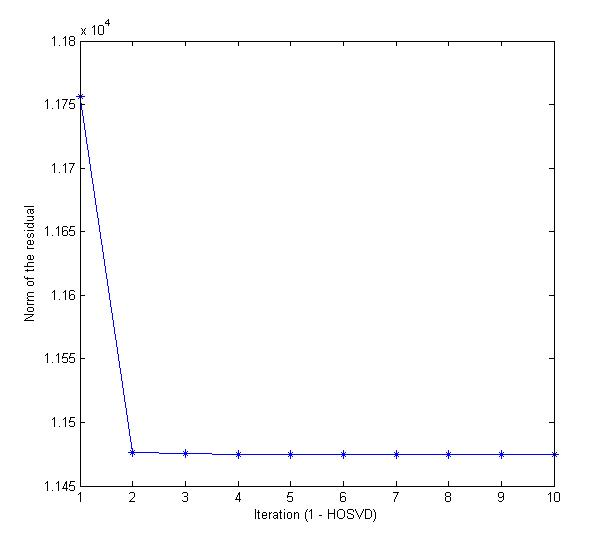
\includegraphics[height=2.3in]{images/hooi_hosvd_residual_plot}
        \caption{Improvement of the norm of the residual, with HOSVD}
    \label{fig:hooiimprove}
\end{figure}


\begin{figure}[ht!]
\centering
        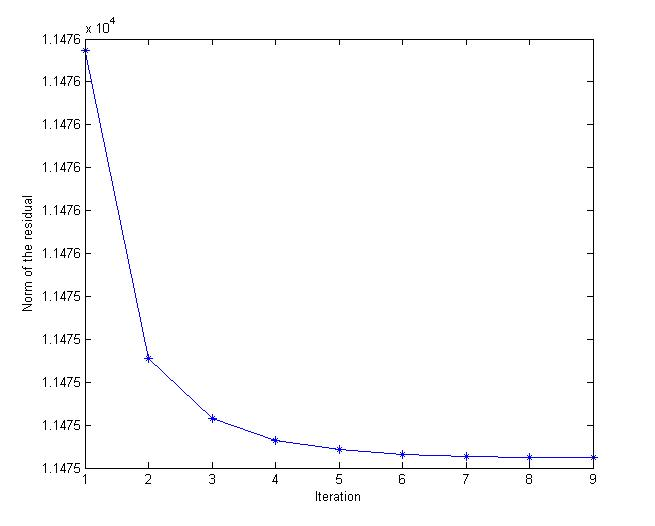
\includegraphics[height=2.3in]{images/hooi_residual_plot}
        \caption{Improvement of the norm of the residual, without HOSVD}
    \label{fig:hooiimprove1}
\end{figure}


The Figure \ref{fig:hooi_grad_plot} shows the dynamics of the
projected gradient. Note that the plot is in logarithmic scale.
We can see that, even though the norm of the residual practically
stopped changing after first $10$ iterations,
the norm of the gradient is decreasing quite fast even at iterations
$30$ to $40$. We conclude that for our data HOOI converges to 
a critical point.

\begin{figure}
        \centering
                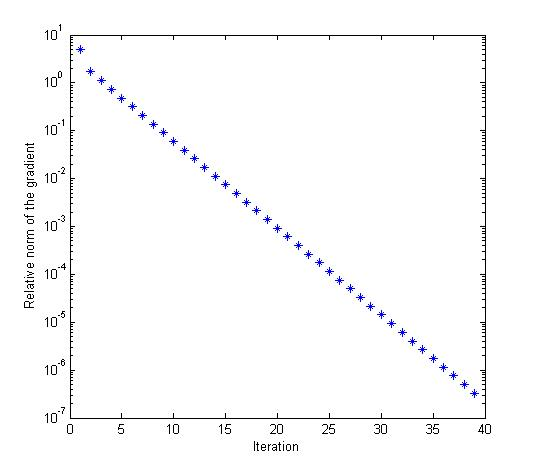
\includegraphics[width=8cm]{images/hooi_gradient_plot.jpg}
        \caption{Relative norm of the gradient (logarithmic scale).}
        \label{fig:hooi_grad_plot}
\end{figure}


As for Newton methods, they demonstrate some very small improvement
during first $4$ or $5$ iterations and then they started
diverging very fast. A typical example (for differential-geometric Newton method) is in Figure \ref{fig:grad_newgr}.
Note that the plot is in logarithmic scale. Due to the non-monotonicity of both Newton methods, in practice we observed
$4$ iterations more to be absolutely sure that this rapid increase is indeed a sign of divergence. 


\begin{figure}
        \centering
                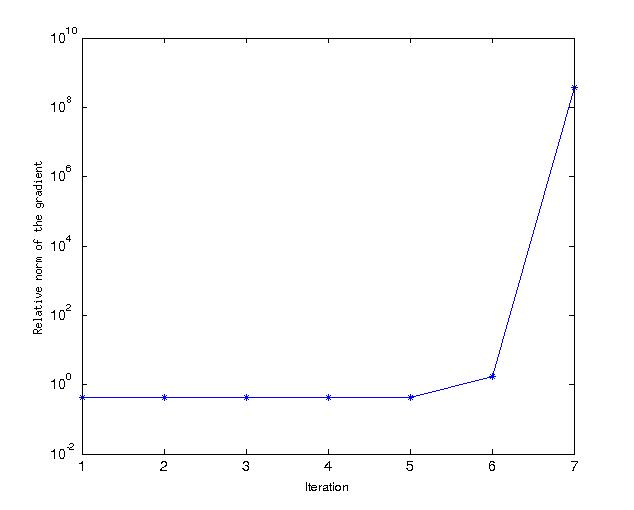
\includegraphics[width=8cm]{images/grad_newgr.jpg}
        \caption{Relative norm of the gradient in Differential-Geometric Newton method (logarithmic scale).}
        \label{fig:grad_newgr}
\end{figure}


\section{Reconstruction and Fitting}
\label{eval_fit}

The more application-relevant measure is fitting error: we take a face scan $\tilde{\f}$
from the testing dataset and try to fit it to the model. Recall the formulation of this from Section \ref{mult_model}.

\begin{equation}
\mbox{Find $\w_2 \in \R^{r_2}$, $\w_3 \in \R^{r_3}$ that minimize } \rho(\tilde{\f}, \f(\w_2, \w_3)) \to \min.
\end{equation}

Here $\f(\w_2, \w_3)$ denotes the reconstructed face $\bmu + \G \times_2 \w_2 \times_3 \w_3$. The fitting error
$\rho$ is defined to be
\begin{equation}
\rho(\tilde{\f}, \f) := \sum_{ p \in \f } dist(p, NN(p, \tilde{\f}),
\end{equation}
where $NN(p, \tf)$ is the nearest neighbour of point $p$ on the scan $\tf$. 


The actual procedure of fitting starts with finding a rigid transformation
that aligns the input scan with the mean face $\bmu$. After alignment
at each iteration the non-linear optimization procedure \textrm{vnl\_lbgfs} from the VNL library
is used to improve the weights.



If the input to the fitting procedure is a registered scan, not a scan from the original
database, then we call this procedure reconstruction. In this case
we wish the model to reproduce the face with the same correspondence. The reconstruction
error is measured by simply computing the distance between the points with the same
index in $\f$ and $\tf$. The reconstruction error is typically higher than the 
fitting error, since it is harder to satisfy the dense correspondence constraint.


The average values of the fitting and reconstruction errors are given in Table \ref{avg_fit_rec_error}.
We can see that there is no significant difference. Interestingly, HOSVD demonstrates
the worst results for fitting and the best results for reconstruction. However,
even though the difference between values of HOSVD and all other methods is more than the difference
between any other two methods, still it is too small to draw any conclusions.



The average values alone do not provide much information. It might be that for some methods
the distribution of errors is significantly different or that some methods perform much better
in certain regions of a face than other methods do. In order to be sure that this is not the case
we produced cumulative error plots and visualized average error per vertex using false colored models.
In Figure \ref{fig:cum_err_reconstruct}
we give the cumulative error plot for reconstruction with Newton-Grassmann method, in Figure \ref{fig:cum_err_fit}
we give the cumulative error plot for fitting with HOOI with $4$ iterations. Of course, the shapes of the curves are quite different, this again demonstrates that reconstruction with correspondence is significantly harder.
However, if we compare two different methods on the same problem, we shall hardly be able to see the difference, 
that is why we give just these two plots and not all $10$ of them.


\begin{table}[h]
\centering
\begin{tabular}{|c|c|c|}
\hline
Method                         & Average reconstruction error, mm & Average fitting error, mm \\ \hline
HOSVD                         & $3.3551 $   &  $ 1.3201 $      \\ \hline
HOOI-4                        & $3.3708$  &  $ 1.3184 $     \\ \hline
HOOI-30                       & $3.37410$   &  $ 1.3179 $     \\ \hline
NG                           & $ 3.3702 $   &  $ 1.3182  $   \\ \hline
DGN                          &  $3.3702 $  &  $ 1.3182 $      \\ \hline
\end{tabular}
\caption{Values of the average reconstruction and fitting errors. HOOI-4 stands for $4$ iterations of HOOI; HOOI-30 stands for $30$ iterations of HOOI; NG stands for Newton-Grassmann method, DGN stands for Differential-Geometric Newton Method.}
\label{avg_fit_rec_error}
\end{table}


\begin{figure}
        \centering
                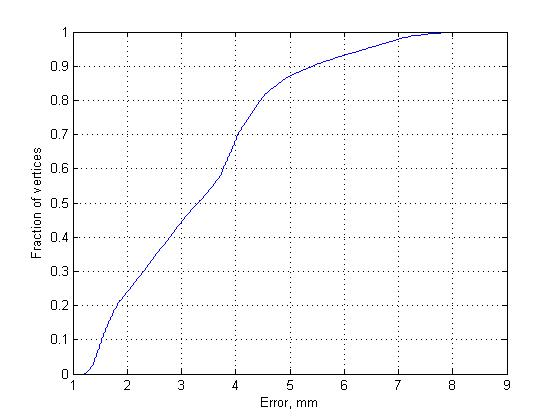
\includegraphics[width=8cm]{images/cum_error_rec_newgr.jpg}
        \caption{Cumulative error plot for reconstruction with Newton-Grassmann. For example, $70 $ \% of all vertices have error less than $4$ mm.}
        \label{fig:cum_err_fit}
\end{figure}

\begin{figure}
        \centering
                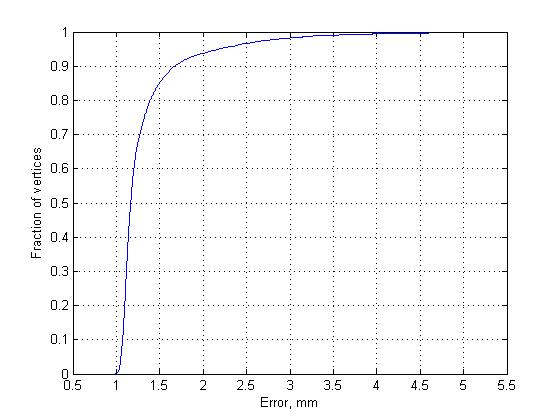
\includegraphics[width=8cm]{images/cum_error_fit_hooi_4.jpg}
        \caption{Cumulative error plot for fitting with HOOI. For example, about $84 $ \% of all vertices have error less than $1.5$ mm.}
        \label{fig:cum_err_fit}
\end{figure}




% In addition, we plot
%the average error per vertex in Figure \ref{avg_fit_rec_error}. The green areas correspond
%to the vertices where the average error is low, the red areas indicate vertices
%where the error is high. There is again no significant difference in the distribution
%of the error on face. 

\section{Expression Recognition}


We consider two approaches to the expression recognition problem.
The first step in both of them is
to fit the input scan $\tf$ to the model and get identity 
and expression weights.  

The most straightforward approach uses a simple nearest-neighbour classification.
We do not fit the scans of the training database to the model, but simply use
the columns of the projection matrix responsible for expression as representatives
of all faces in the training dataset that have this expression. This gives us $24$ (we ignore neutral
expression)
points in $\R^7$. We take the expression weight of the testing scan, search for
its nearest neighbour among these $24$ points and return the corresponding expression.
Maybe, it would be more accurate to actually fit the training scans
to the model and then we would have much more samples in the expression space.
However, fitting takes time and, more importantly, its 
results heavily depend on the initialization. If we choose
the corresponding column of the projection matrix
as an initial expression weight for fitting procedure (which 
seems to be a very reasonable choice), we should
get the final expression weight that is not too 
far way from this initial value.


The more involved approach was inspired by Mpiperis et al. \cite{mpip_2008}.
Before we start classification, we reconstruct the original faces using the learnt model.
Let $\G$ be the core tensor of the model, $F_2$ and $F_3$ be the projection matrices. The reconstructed
faces are (by definition) sums of the mean face $\bmu$ and mode-$1$ fibers of the tensor $\G \times_2 F_2^T \times_3 F_3^T$.

Now let $\f$ be an input scan from the testing dataset. The fitting procedure
gives us the identity and expression weights $\w_2$, $\w_3$. We can now reconstruct
the approximate version of $\f$ using the model as
\begin{equation}
\tf := \bmu + \G \times_2 \w_2^T \times_3 \w_3^T.
\end{equation}
Now each of the reconstructed faces of the training dataset casts a vote for its expression.
The vote is a real number proportional to $\exp( - d^2 / \sigma)$. Here $d$ is the
distance between the reconstructed face from the training dataset and $\tf$,
and $\sigma$ is some constant. All votes are summed up, and the expression
that obtained the maximal sum of votes is returned as the output
of the classification procedure.


In fact, we were slightly inaccurate when said that $d$ is the distance 
between $\tf$ and a reconstructed face from the training dataset. There are many
points that are not relevant for many expressions, and the noise from them,
when added up, may confuse the classifier. Instead of measuring distance
between all the corresponding points in both faces, only a subset is chosen
and the distances between corresponding points from that subset are added up
to make $d$.




\begin{table}[h]
\centering
\begin{tabular}{|l|l|l|l|l|l|l|}
\hline
Ground Truth\\Classified as    & Angry & Disgust & Fear & Happy & Sad & Surprised \\ \hline


Angry     &  	 54.50 	 &  11.00 	 &  8.25 	 &  2.25 	 &  23.00 	 &  1.00 \\ 
Disgust   &  	 29.25 	 &  44.00 	 &  12.00 	 &  3.75 	 &  6.75 	 &  4.25 \\ 
Fear      &  	 18.50 	 &  6.75 	 &  32.50 	 &  18.50 	 &  18.00 	 &  5.75 \\ 
Happy     &  	 23.00 	 &  4.75 	 &  23.25 	 &  38.75 	 &  6.00 	 &  4.25 \\
Sad       &  	 26.25 	 &  7.25 	 &  14.75 	 &  1.75 	 &  49.00 	 &  1.00 \\
Surprised &  	 25.25 	 &  2.25 	 &  6.50 	 &  4.50 	 &  27.75 	 &  33.75 \\ \hline

\end{tabular}
\caption{Confusion matrix for expression recognition, HOSVD }
\label{expr_rec_hosvd_confmatr_nn}
\end{table}


\begin{table}[h]
\centering
\begin{tabular}{|l|l|l|l|l|l|l|}
\hline
Ground Truth\\Classified as    & Angry & Disgust & Fear & Happy & Sad & Surprised \\ \hline

Angry     &  	 53.25 	 &  11.50 	 &  9.50 	 &  1.00 	 &  24.75 	 &  0.00 \\
Disgust   &  	 28.25 	 &  47.50 	 &  10.50 	 &  3.75 	 &  6.75 	 &  3.25 \\
Fear      &  	 20.75 	 &  8.50 	 &  33.25 	 &  13.75 	 &  16.50 	 &  7.25 \\
Happy     &  	 19.00 	 &  8.00 	 &  25.75 	 &  38.25 	 &  4.75 	 &  4.25 \\
Sad       &  	 21.25 	 &  7.50 	 &  14.25 	 &  2.00 	 &  54.25 	 &  0.75 \\
Surprised &  	 20.25 	 &  1.75 	 &  8.00 	 &  5.25 	 &  30.50 	 &  34.25 \\ \hline
\caption{Confusion matrix for expression recognition, HOOI, 4 iterations }
\label{expr_rec_hooi_confmatr_nn}
\end{table}


\begin{table}[h]
\centering
\begin{tabular}{|l|l|l|l|l|l|l|}
\hline
Ground Truth\\Classified as    & Angry & Disgust & Fear & Happy & Sad & Surprised \\ \hline
Angry     &  	 49.25 	 &  11.75 	 &  9.50 	 &  1.50 	 &  27.75 	 &  0.25 \\
Disgust   &  	 31.00 	 &  44.75 	 &  9.00 	 &  4.00 	 &  7.75 	 &  3.50 \\
Fear      &  	 20.00 	 &  8.25 	 &  32.75 	 &  14.50 	 &  18.00 	 &  6.50 \\
Happy     &  	 17.25 	 &  7.25 	 &  23.50 	 &  42.00 	 &  5.50 	 &  4.50 \\
Sad       &  	 23.50 	 &  7.25 	 &  11.75 	 &  1.75 	 &  54.00 	 &  1.75 \\
Surprised &  	 19.50 	 &  3.25 	 &  6.75 	 &  5.00 	 &  35.50 	 &  30.00 \\ \hline

\caption{Confusion matrix for expression recognition, HOOI, 30 iterations }
\label{expr_rec_hooi_30_confmatr_nn}
\end{table}


\begin{table}[h]
\centering
\begin{tabular}{|l|l|l|l|l|l|l|}
\hline
Ground Truth\\Classified as    & Angry & Disgust & Fear & Happy & Sad & Surprised \\ \hline
Angry     &  	 52.50 	 &  12.00 	 &  9.25 	 &  1.00 	 &  25.25 	 &  0.00 \\
Disgust   &  	 30.50 	 &  46.25 	 &  10.00 	 &  3.75 	 &  6.25 	 &  3.25 \\
Fear      &  	 20.00 	 &  7.50 	 &  34.50 	 &  14.25 	 &  16.75 	 &  7.00 \\
Happy     &  	 18.75 	 &  7.00 	 &  27.25 	 &  38.25 	 &  4.50 	 &  4.25 \\
Sad       &  	 21.75 	 &  7.75 	 &  13.25 	 &  2.00 	 &  54.50 	 &  0.75 \\
Surprised &  	 20.25 	 &  2.25 	 &  8.00 	 &  5.50 	 &  29.75 	 &  34.25 \\

\end{tabular}
\caption{Confusion matrix for expression recognition, Newton-Grassmann}
\label{expr_rec_newgr_confmatr_nn}
\end{table}


\begin{table}[h]
\centering
\begin{tabular}{|l|l|l|l|l|l|l|}
\hline
Ground Truth\\Classified as    & Angry & Disgust & Fear & Happy & Sad & Surprised \\ \hline
Angry     &  	 53.50 	 &  12.50 	 &  10.75 	 &  0.75 	 &  22.25 	 &  0.25 \\
Disgust   &  	 30.50 	 &  46.50 	 &  11.25 	 &  2.50 	 &  6.00 	 &  3.25 \\
Fear      &  	 20.75 	 &  9.00 	 &  32.25 	 &  15.00 	 &  16.75 	 &  6.25 \\
Happy     &  	 20.00 	 &  5.75 	 &  28.50 	 &  37.75 	 &  4.25 	 &  3.75 \\
Sad       &  	 22.75 	 &  8.25 	 &  13.50 	 &  2.00 	 &  52.75 	 &  0.75 \\
Surprised &  	 19.50 	 &  1.75 	 &  8.00 	 &  5.00 	 &  30.00 	 &  35.75 \\ \hline
\end{tabular}
\caption{Confusion matrix for expression recognition, Differential-Geometric Newton}
\label{expr_rec_dg_newton_confmatr_nn}
\end{table}

\begin{table}[h]
\centering
\begin{tabular}{|c|l|l|l|l|l|}
\hline
                            Method              & HOSVD & HOOI-4 & HOOI-30 & NG & DGN \\ \hline
Classification rate, NN, \%                         & $42.0833$  & $43.4583$ & $42.125$ & $ 43.375 $ & $43.0833$ \\ \hline
Classification rate, with reconstruction            & $ 40.25 $  & $39.75 $  & $ 37.7917$ & $ 39.7083$ & $39.875 $ \\ \hline
\end{tabular}
\caption{Expression recognition rate, comparison}
\label{expr_rec_rate_total}
\end{table}


\chapter{Conclusion}




\bibliography{biblio1}{}
\bibliographystyle{plain}
\end{document}
